\documentclass[czech, bachelor]{diploma}
\usepackage[autostyle=true, czech=quotes]{csquotes}
\usepackage{dcolumn}
\usepackage{subfig}
\usepackage{hyperref}
\usepackage{xurl}
\usepackage{listings}
\PassOptionsToPackage{usenames,dvipsnames}{xcolor}

% A protože jsem namyšlený, pojmenuju to podle sebe
\newcommand{\filipref}[1]{\ref{#1}\,--\,\nameref{#1}}

% Propůjčeno z https://github.com/cansik/kotlin-latex-listing
% Geniální člověk co používá skvělý jazyk
\lstdefinelanguage{Kotlin}{
  comment=[l]{//},
  commentstyle={\color{gray}\ttfamily},
  emph={filter, first, firstOrNull, forEach, lazy, map, mapNotNull, println},
  %emphstyle={\color{OrangeRed}},
  emphstyle=\color{orange},
  %identifierstyle=\color{black},
  identifierstyle=\color[RGB]{43,145,175},
  keywords={!in, !is, abstract, actual, annotation, as, as?, break, by, catch, class, companion, const, constructor, continue, crossinline, data, delegate, do, dynamic, else, enum, expect, external, false, field, file, final, finally, for, fun, get, if, import, in, infix, init, inline, inner, interface, internal, is, lateinit, noinline, null, object, open, operator, out, override, package, param, private, property, protected, public, receiveris, reified, return, return@, sealed, set, setparam, super, suspend, tailrec, this, throw, true, try, typealias, typeof, val, var, vararg, when, where, while},
  %keywordstyle={\color{NavyBlue}\bfseries},
  keywordstyle=\color{blue},
  morecomment=[s]{/*}{*/},
  morestring=[b]",
  morestring=[s]{"""*}{*"""},
  ndkeywords={@Deprecated, @JvmField, @JvmName, @JvmOverloads, @JvmStatic, @JvmSynthetic, Array, Byte, Double, Float, Int, Integer, Iterable, Long, Runnable, Short, String},
  %ndkeywordstyle={\color{BurntOrange}\bfseries},
  ndkeywordstyle=\color{blue},
  sensitive=true,
  stringstyle=\color[RGB]{163,21,21}
  %stringstyle={\color{ForestGreen}\ttfamily},
}

\lstdefinelanguage{OstraJava}{
  comment=[l]{//},
  commentstyle={\color{gray}\ttfamily},
  emph={fajront, banik, pyco, Ostrava, rynek, toz, naDryst, kantuje},
  emphstyle=\color{orange},
  identifierstyle=\color[RGB]{43,145,175},
  keywords={fajne, nyt, chuj, kaj, kajtez, boinak, rubat, zdybat, dlabat, davaj, zrob, forant, tryda, fagan, od, ci, aj},
  keywordstyle=\color{blue},
  morecomment=[s]{/*}{*/},
  morestring=[b]",
  morestring=[s]{"""*}{*"""},
  ndkeywords={cyslo, bul, chachar, cyslo\_desetinne, Dryst, Bazmek, Citac, Konzola, Bafr},
  ndkeywordstyle=\color{blue},
  sensitive=true,
  stringstyle=\color[RGB]{163,21,21}
}

\ThesisAuthor{Filip Peterek}
\ThesisSupervisor{Ing. Jan Gaura, Ph.D.}
\CzechThesisTitle{Vývoj samoříditelné platformy}
\EnglishThesisTitle{Self-driving Platform Development}
\SubmissionYear{2021}

\Acknowledgement {
    Chtěl bych poděkovat vedoucímu mé práce, Janu Gaurovi, nejen za pomoc s tvorbou práce a~návrhem softwaru, ale především
    za možnost se projevit a pracovat na skutečném a zajímavém projektu. Dále chci poděkovat svým kolegům z práce, kteří mě
    naučili spoustu věcí, na které v~akademickém prostředí není čas nebo příležitost.
}

\CzechAbstract {
    Tato práce se zabývá vývojem softwaru pro samořiditelnou platformu vznikající na VŠB-TUO. Po~dokončení by software měl být
    schopen na základě vstupů ze softwaru pro analýzu obrazu, GPS, Lidaru a řídící jednotky vozidla bezpečně navigovat autonomní
    platformu univerzitním kampusem.

    Řídící software je rozdělen do dvou komponent. První komponenta zajišťuje komunikaci s řídící jednotkou vozidla pomocí
    sběrnice CAN, na starosti má ovládání rychlosti vozidla a natáčení kol. Druhá komponenta má na starosti plánování cesty
    na základě výše vyjmenovaných vstupů. První komponentě poté zadá pouze požadovanou rychlost vozidla a natáčení kol, samotné
    posílání CAN zpráv však nemusí řešit. Komponenty mezi sebou komunikují pomocí protokolu TCP. K testování ovládacího software
    lze využít simulátor, který dokáže nasimulovat chování první komponenty. Pro~řízení vozidla jsou v hojné míře využívány PID
    regulátory.

    V době odevzdání této práce ještě není software plně dokončený, jelikož se jedná o výzkumný projekt, který svým rozsahem
    přesahuje bakalářskou práci, a vývoj platformy bude dále pokračovat.
}

\CzechKeywords {
    plánování cesty, client-server komunikace, sběrnice CAN, PID regulátor
}

\EnglishAbstract {
    This thesis is focused on the development of software for a self-driving platform, which is being developed by the Technical
    University of Ostrava. Upon completion, the software should be capable of safely navigating an autonomous vehicle through
    the university campus, taking inputs from image analysis software, GPS, Lidar, and the~vehicle's own controller unit.

    The software is split into two components. The first component handles communication with the~vehicle's controller
    unit via a CAN bus. The second component then does all the path planning, taking into account the aforementioned inputs.
    The second component then asks the first component to maintain a certain speed or steer the vehicles, however, it doesn't
    have to handle CAN messages, including driving inputs or control checksums, by itself. The TCP protocol is~used
    for communication between the components. The path planning software can be tested using a~simulator, capable of mocking
    the CAN handling software, along with the entire vehicle. The~simulator honors the~TCP API, however, the vehicle physics
    are simplified. PID controllers are used in~multiple parts of~the software.

    At the time of publishing this paper, the software is still unfinished, as the self-driving platform is an academic research
    project, which outspans this bachelor's thesis in scope, and development of~the~platform will continue.
}

\EnglishKeywords {
    path planning, client-server communication, CAN bus, PID controller
}

\AddAcronym{CAN}{Controller Area Network}
\AddAcronym{PID}{Proporcionální-integrační-derivační}
\AddAcronym{TCP}{Transmission Control Protocol}
\AddAcronym{GPS}{Global Positioning System}
\AddAcronym{API}{Application Programming Interface}
\AddAcronym{XML}{Extensible Markup Language}
\AddAcronym{JSON}{JavaScript Object Notation}
\AddAcronym{YAML}{YAML Ain't a Markup Language}
\AddAcronym{TX}{Transmitter}
\AddAcronym{RX}{Receiver}
\AddAcronym{RPC}{Remote Procedure Call}
\AddAcronym{REST}{Representational state transfer}
\AddAcronym{OSM}{OpenStreetMap}
\AddAcronym{URL}{Uniform Resource Locator}

% Novy druh tabulkoveho sloupce, ve kterem jsou cisla zarovnana podle desetinne carky
% Já jako chápu, jaký je význam tohoto, ale bylo to v šabloně od Dvorského, nikde to (momentálně) nevyužívám
% Možná to zapomenu smazat
% TODO: Smazat, jestli to nevyužiju.
\newcolumntype{d}[1]{D{,}{,}{#1}}

\begin{document}

\MakeTitlePages

\chapter{Úvod} \label{sec:Introduction}
Tato práce je součást většího výzkumného projektu. Cílem projektu je vývoj autonomního eletrifikovaného vozidla,
od fyzického návrhu a zkonstruování vozidla, až po vývoj softwaru. Hotové vozidlo má být schopno plně autonomního pohybu
po univerzitním kampusu, kde má sloužit k rozvozu materiálu napříč budovami. Při tvorbě samořiditelné platformy je nutné
klást vysoký důraz na bezpečnost provozu, výsledek projektu při reálném využití nesmí ohrozit zdraví ani majetek
univerzity nebo jejích návštěvníků.

Samotná práce se zabývá vývojem řídícího softwaru vozidla. Software bude sloužit k navigaci vozidla areálem univerzity,
plánování cesty, a zajištění bezpečnosti provozu. Pro tento účel řídící kód využívá vstupy z GPS, kamer, Lidaru,
a ovládací jednotky vozidla. Analýza obrazu a dat naměřených Lidarem není předmětem této práce, výsledek této analýzy
je získáván z API komponenty určené právě k tomuto účelu, taktéž vyvíjené jako součást projektu.

Software, který je vyvíjen jako součást této práce, je tvořen v Pythonu, a je rozdělen do více komponent. Kromě řídícího
softwaru byl vyvinut také jednoduchý simulátor, umožňující testování řízení. Dále řídící software obsahuje funkční
vizualizér, pomocí kterého je možné sledovat pohyb vozidla. Při tvorbě řídících komponent byla využita řada open source
knihoven a veřejných zdrojů, včetně map OpenStreetMap nebo Mapy.cz. Zdrojový kód, který je součástí této práce, je
rovněž otevřený a veřejně dostupný na Githubu \cite{car-client-source, car-webapp-source, car-map-downloader-source,
car-can-source, car-simulator-source, geologger-source}.

\chapter{Architektura řídícího softwaru} \label{software-architecture}
Jak již bylo zmíněno, řídící software je rozdělen do dvou komponent, komunikujících mezi sebou pomocí protokolu TCP na bázi
architektury klient-server. Jako server slouží program zajišťující přenos dat na rozhraní CAN. Server takto abstrahuje
nízkoúrovňové a bezpečnostní záležitosti, mezi které patří výpočet kontrolních součtů, zasílání CAN zpráv, TX/RX synchronizace,
žádání o~možnost ovládat vozidlo, regulace rychlosti pomocí PI regulátoru, nebo také zpracování výstupu z~GPS modulu. Klient tak
může implementovat pouze samotné plánování cesty, v dotazech na~server stačí žádat pouze o dodržování rychlosti, úhlu natočení
kol, případně aplikace nouzové brzdy. Server samozřejmě dokáže poskytovat zpětnou vazbu, tedy informace o aktuální rychlosti,
pozici, natočení kol, nebo zdraví systému (tzv. \emph{healthcheck}). Server je většinou spouštěn na Raspberry~Pi, ačkoliv může
být spouštěn na libovolné jednotce připojené k rozhraní CAN samořiditelné platformy, za~předpokladu, že je na dané jednotce
nainstalován interpreter jazyka Python.

Toto dělení nejen zvyšuje úroveň abstrakce, a tím i čitelnost kódu, ale zároveň umožňuje spustit program plánující
cestu vozidla na vzdáleném stroji. Takto můžeme například program spouštět na~výkonnějším stroj a vyhnout se omezením
Raspberry~Pi, virtualizovat ovládací software, nebo implementovat jiný typ klienta, které v současné době existují tři.
Jeden klient se snaží vozidlo řídit na základě vstupů ze senzorů umístěných na vozidle a z komponenty určené pro analýzu obrazu.
Druhý klient umožňuje řídící pokyny zadávat manuálně do jednoduchého textového prostředí. Třetí klient poté pouze pošle
předdefinovanou testovací sekvenci. Druhý a třetí klient jsou určeny pouze k~ověření funkčnosti komunikace pomocí sběrnice CAN.
Virtualizace ovládacího softwaru také umožňuje zautomatizovat monitorování ovládání. Ačkoliv k žádným pokusům o automatickou
orchestraci a monitorování zatím nedošlo, bylo by možné například spouštět řídící software v Kubernetes, nastavit kontinuální
nasazování pomocí CI/CD pipeline, a logy či metriky kontrolovat strojově pomocí nástrojů jako ELK stack nebo Prometheus.

\chapter{Server a CAN komunikace}

TCP server slouží k vzdálenému ovládání vozidla pomocí libovolného klienta. Software serveru je~spouštěn na zařízení Raspberry~Pi
připojeném k rozhrání CAN autonomní platformy. CAN komunikace je implementována za využití knihovny \emph{python-can} a software
je schopen vozidlu předávat pokyny a zároveň vozidlo regulovat a monitorovat. Sám ale nedokáže plánovat cestu nebo reagovat
na vnější události ovlivňující vozidlo, dokáže však zpracovat interní chyby. Software tedy slouží čistě a pouze ke zpracování
interních záležitostí vozidla.

Architektura softwaru a důvod dělení na server a klient jsou podrobněji popsány v kapitole \filipref{software-architecture}.

\section{Sběrnice CAN}

Controller Area Network \cite{can-source}, zkráceně CAN, je standard poskytující určitý základ pro komunikaci na~sběrnici.
Standard definuje fyzické požadavky na sběrnici a formát zpráv. Součástí zprávy je~osm bytů vyhrazených pro data. Sběrnice CAN je,
mimo jiné, hojně využívána právě v~automobilovém průmyslu.

\subsection{Vlastní specifikace}
Standard sice přiřazuje každé zprávě pole o velikosti osm bytů vyhrazené pro data, již však nedefinuje, jaká data mají zprávy
obsahovat, v jakém formátu mají být data posílána, nebo jak se s~nimi má pracovat \cite{can-source}. Obsah zpráv tak musel být
vydefinován vlastní specifikací, která prošla hned několika iteracemi, a jejíž finální podoba je výsledkem úzké spolupráce
konstruktérů fyzické platformy a tvůrců řídícího softwaru. Specifikace byla navrhována tak, aby umožnila dostatečně jemné řízení
vozidla, poskytovala řídícímu softwaru všechna potřebná jízdní data a zahrnovala množství prostředků pro kontrolu integrity
zprávy, rychlé zachycení chyb či reportování problémů. Na~chyby nebo problémy je samozřejmě důležité reagovat, v krajních
případech až nouzovým zastavením vozidla. Software pro ovládání platformy byl již několikrát přepisován na základě upravené
specifikace, nejaktuálnější verze softwaru však implementuje nejnovější verzi specifikace. Ukázku části specifikace si lze
prohlédnout v tabulce \ref{tab:can-spec-table}.

\begin{table}
  \centering
  \caption{Ukázka současné verze vlastní CAN specifikace}
  \label{tab:can-spec-table}
  \begin{tabular}{ |c|c|c|c|c|c|c| }
    \hline
    Message Name     & ID  & Cycle (ms) & Byte & Length (bits) & Min Value & Max Value \\
    \hline
    System Status    & 201 & 20         & 1    & 1             & 0         & 1 \\
    \hline
    Control Request  & 201 & 20         & 2    & 1             & 0         & 1 \\
    \hline
    Steering Request & 201 & 20         & 3    & 8             & 0         & 255 \\
    \hline
    Drive Request    & 201 & 20         & 4    & 8             & 0         & 255 \\
    \hline
    Drive Gain       & 201 & 20         & 5    & 2             & 0         & 4 \\
    \hline
    Steering Gain    & 201 & 20         & 6    & 2             & 0         & 4 \\
    \hline
    Message Count    & 201 & 20         & 7    & 8             & 0         & 255 \\
    \hline
    Data Checksum    & 201 & 20         & 8    & 8             & 0         & 255 \\
    \hline
  \end{tabular}
\end{table}

Specifikace, kromě formátu a obsahu dat, určuje také formát, jakým je kódována rychlost vozidla nebo natočení předních kol. Tyto
hodnoty jsou kódovány a uloženy v jednom bytu. Při práci s~CAN sběrnicí tak je nutné data správně přepočíst a zakódovat, případně
dekódovat a převést do formátu IEEE 754.

\section{TCP server a jeho metody} \label{server-methods}

Za účelem zvýšení úrovně abstrakce a zjednoduššení ovládání vozidla, ale také aby bylo umožněno vzdálené ovládání platformy
a zjednodušila se výměna způsobů ovládání, je nízkoúrovňové řízení CAN zprávami abstrahováno a obaleno jednoduchým TCP serverem.
Při vývoji serveru se přirozeně nabídla možnost implementace REST API a využití protokolu HTTP, nebo využití jednoho z rozšířených
RPC prokolů, jako jsou XMLRPC nebo gRPC. Ačkoliv validní, tyto způsob, implementace se jevily jako neefektivní -- rozhraní
poskytované serverem je velmi jednoduché, plaintextový protokol HTTP nebo variace protokolů RPC tak působily až zbytečně
komplikovaně. Pro komunikaci byl nakonec použit vlastní binární protokol a jeho implementace přímo nad TCP sockety.
Výhodou je rychlost a~jednoduchost implementace, úspornost a výkonnost řešení v reálném provozu, nebo také fakt, že toto řešení
nevyžaduje žádné externí závislosti nad rámec standardní knihovny jazyka Python. Nevýhody současného řešení by se projevily
pouze při výrazném nárůstu komplexity poskytovaného rozhraní. Tento scénář by mohl vést k znepřehlednění současného řešení.
Nutnosti zvyšování komplexity rozhraní ovšem v současné době nic nenasvědčuje.

Aktuální verze serveru implementuje celkem pět metod. Na vstupu přijímá celkem tři byty. První byte je vyhrazen pro identifikaci
metody serveru. Následující dva byty dotazu obsahují data. Klient musí vždy poslat minimálně tři byty, na vstupu jsou, nezávisle
na metodě, pokaždé očekávány tři byty. Jestliže klient pošle v dotazu více než dva datové byty, budou nadbytečná data ignorována.

Jako identifikátor metody je využito celé nezáporné číslo. V případě, že první byte zprávy obsahuje identifikátor nepříslušící
žádné metodě, je dotaz ignorován. Obsah datových bytů je určen danou metodou serveru. Pokud pro danou funkcionalitu není třeba
předávat serveru žádná data, může být obsah datových bytů libovolný, data budou ignorována.

\subsection{Metoda \emph{drive}}
Metoda \emph{drive} slouží k předání požadované rychlosti vozidla a natočení kol. Obsah první datového bytu je interpretován jako
rychlost, druhý datový byte reprezentuje natočení předních kol. Oba datové byty jsou interpretovány jako celá znaménková čísla.

Fyzická změna rychlosti nebo natočení kol samozřejmě nemůže nastat okamžitě, rychlost změny je omezena fyzikálními vlastnostmi
konstrukce i PI regulátorem, proto nelze vrátit klientu potvrzení o provedené změně. Odpovědí metody je ekvivalentní s metodou
\emph{healthcheck}. \emph{Healthcheck} v odpovědi slouží jako potvrzení přijetí dotazu a schopnosti dotazu vyhovět. V případě,
že klient potřebuje potvrzení o dosažení požadované rychlosti nebo úhlu natočení kol, je možné po zavolání metody \emph{drive}
opakovaně volat metodu \emph{info}.

\subsection{Metoda \emph{healthcheck}}
Metoda \emph{healthcheck} slouží k ověření \emph{živosti} systému. \emph{Živost} je binární stav, systém je buď \emph{živý}, nebo
\emph{mrtvý}. Server je považován za \emph{živý}, jestliže je schopen zpracovávat TCP spojení, a zároveň má plnou kontrolu
nad vozidlem. V opačném případě je server považován za \emph{mrtvý}. Metoda nepřijímá žádný vstup, datové byty jsou ignorovány.

\emph{Healthcheck} ve své odpovědi posílá pouze jeden byte. Pokud je server živý, obsahuje odpověď nenulovou hodnotu. V opačném
případě vrátí server nulu, nebo neodpoví vůbec.

\subsection{Metoda \emph{info}}
\emph{Info} metoda TCP serveru se využívá k získání aktuálních jízdních dat vozidla. Na vstupu nepřijímá žádné parametry, všechny
datové byty jsou tedy ignorovány. Na výstupu server vrátí tři byty. První dva byty reprezentují znaménková celá čísla. Obsahem
prvního bytu je aktuální rychlost vozidla. Druhý byte obsahuje úhel natočení kol. Poslední byte poté obsahuje logickou hodnotu
značící stav nouzové brzdy. Jestliže je hodnota třetího bytu nulová, nouzová brzda není aktivována. Nenulová hodnota značí,
že došlo k aktivaci nouzového brždění, a bude třeba jej deaktivovat, pokud chceme pokračovat v jízdě.

\subsection{Metoda \emph{ebrake}}
\emph{Ebrake}, nebo-li \emph{'Emergency Brake'}, česky 'nouzová brzda', slouží k ovládání nouzového brždění. První byte vstupu
je serverem interpretován jako logická hodnota značící požadovaný stav nouzové brzdy. Nenulovou hodnotu server považuje za signál
k aktivaci nouzového brždění. Při přijetí nulové hodnoty na vstupu poté dochází k deaktivaci nouzové brzdy. Druhý byte vstupu
je ignorován.

Výstup metody \emph{ebrake} je opět ekvivalentní výstupu metody \emph{healthcheck}. Nenulová hodnota na~výstupu značí, že server
požadavek přijal a je schopen jej zpracovat. Nula reprezentuje stav, kdy server nemá kontrolu nad vozidlem a není schopen
nouzovou brzdu aktivovat. Pokud však ke~ztrátě kontroly došlo důsledkem chyby, vozidlo začne nouzově brzdit samo.

\subsection{Metoda \emph{position}}

\emph{Position} využijeme, chceme-li zjistit geografickou polohu vozidla. Tato metoda, která neakceptuje žádný vstup, ve svém
17 bytovém výstupu vrací tři hodnoty.

První byte obsahuje logickou hodnotu značící, zda je geografická poloha věrohodná. Nulový byte značí polohu nevěrohodnou,
nenulový byte věrohodnou. Poloha je považována za nevěrohodnou např. pokud nedojde ke správné inicializaci vozidla, GPS modul
nedokáže zaměřit pozici, apod.

V následujících osmi bytech je zakódována zeměpisná šířka (latitude), v posledních osmi bytech pak zeměpisná délka (longitude).
Ačkoliv se jedná o desetinná čísla, pro zjednodušení jsou zakódována jako čísla celá. Skutečná hodnota zeměpisné šířky a délky
je vynásobena číslem $10^{10}$ a převedena na celé číslo. Výsledné číslo je poté odesláno ve formátu little endian. Při zpracování
odpovědi serveru si tedy klient musí dát pozor na endianitu a správně dekódovat přijatou hodnotu.

\section{Regulace PI regulátorem} \label{pi-controller}
Elektrický motor vozidla samozřejmě koncept rychlosti nezná. Elektrický motor je schopen vydávat určitý točivý moment, o který
je samozřejmě možné si zažádat. Mezi točivým momentem a~rychlostí vozidla ovšem neexistuje lineární závislost. Rychlost vozidla
může ovlivnit více faktorů. Např. při~vysokém konstatním točivém momentu na vodorovné nebo svažující se vozovce by vozidlo mohlo
neustále zrychlovat, minimálně dokud by nedosáhlo rychlosti nebezpečné nejen pro samotnou platformu, ale především pro své okolí.
Naopak při stoupání by vozidlo mohlo na rychlosti ztrácet.

O vydání určitého točivého momentu je možné požádat za pomoci CAN sběrnice. Řídící software vyšle CAN zprávu s požadovanou
rychlostí. Kontrolní jednotka vozidla zprávu zpracuje, zkontroluje, a předá požadavek elektromotoru, který upraví svůj výstup.
Při ovládání vozidla ovšem není určování momentu vhodné. Podstatně jednodušší by bylo žádat o dodržování konkrétní rychlosti,
ne momentu. Proto je točivý moment třeba regulovat. A právě zde se jako řešení nabízí využití PI regulátoru
\cite{pid-controller-source}.

Regulátor je zabudován do zdrojového kódu serveru a je implementován softwarově. TCP server na vstupu metody \emph{drive} dostane
požadavek na udržování rychlosti. Server metodu zpracuje a předá regulátoru jako požadovanou hodnotu. Druhým vstupem regulátoru
je aktuální rychlost, kterou lze nalézt v CAN zprávách kontrolní jednotky platformy. Na svém výstupu regulátor vrací požadovaný
moment, který řídící program předá vozidlu pomocí sběrnice CAN.

Proporcionální složka regulátoru slouží ke změně točivého momentu na základě odchylky naměřené rychlosti od rychlosti požadované.
Integrační složka regulátoru slouží ke sčítání předchozích odchylek a k udržování určité hladiny momentu, aby např. při dosažení
požadované rychlosti, kdy~odchylka bude rovna nule, nedošlo k vypnutí motoru. Derivační složka není v této aplikaci potřeba, proto
je využit pouze PI regulátor.

Regulováno je i natočení kol. Zde je regulátor využit zejména k zabránění velkých skokových změn v požadavku na natočení kol. Není
žádoucí, aby požadovaný úhel například rychle osciloval mezi hodnotami -20 a 20 stupňů. PI regulátor zde slouží právě k zajištění
pozvolné změny požadavku. Požadovaný úhel natočení kol je na CAN sběrnici zadáván ve stupních, aplikace regulátoru je zde velmi
jednoduchá.

\section{Python implementace}

Pro implementaci kódu byl zvolen jazyk Python 3.6. Server má pouze dvě externí závislosti, a~to knihovny \emph{python-can} a
\emph{gpsd-py3}. Dále je samozřejmě extenzivně využívána standardní knihovna jazyka Python.

\subsection{Konfigurace}
Ke konfiguraci komponenty jsou využívány systémové enviromentální proměnné, a to zejména kvůli jednoduchosti řešení a konzistence
s ostatními komponentami. Jelikož je program spouštěn pouze na Raspberry~Pi fyzicky připojenému ke CAN sběrnici vozidla,
k virtualizaci pomocí orchestračních nástrojů, jako je třeba Kubernetes, pravděpodobně nikdy nedojde. Argument o jednoduchosti
konfigurace za využití proměnných prostředí při virtualizaci tak u této komponenty neplatí.

\subsection{TCP server}
K vytvoření TCP serveru byl využit modul \emph{socketserver}, který náleží ke standardním modulům patřícím do jazyka Python.
Server funguje na synchronní bázi a na zpracování probíhá pouze na~jednom vlákně. K serveru je v jednom momentě připojen vždy jen
jeden klient, jenž posílá pouze relativně malé množství dotazů. Asynchronní nebo vícevláknová implementace tak není potřeba,
pouze by~zapříčinila znepřehlednění kódu, a to s velmi nízkými až dokonce žádnými benefity. Server naslouchá na konfigurovatelném
portu. Instanci rozhraní vozidla nebo port lze serveru předat parametrem při~inicializaci. Pokud tak uživatel neučinní, rozhraní
vozidla je vytvořeno automaticky a~číslo portu je~vyčteno z enviromentální proměnné \emph{SERVER\_PORT}.

\subsection{Rozhraní vozidla}
Rozhraní vozidla, v kódu třída \emph{Car}, představuje abstrakci nad sběrnicí CAN, a to aby samotný TCP server nemusel pracovat
přímo s CAN zprávami. Instance třídy \emph{Car} umožňují TCP serveru nastavovat nebo získávat hodnotu úhlu zatočení předních kol,
rychlost, záchrannou brzdu, případně získat GPS pozici vozidla, aniž by TCP server musel počítat s momentem, CAN hodnotami, nebo
pracovat s hardwarovými moduly.

Za účelem práce s CAN sběrnicí byly implementovány třídy \emph{Transmitter} a \emph{Receiver}, které slouží k přijímání a vysílání
zpráv. Interně třídy využívají prostředky poskytované modulem \emph{python-can}, zvenčí představují především abstrakci
nad nízkoúrovňovými CAN záležitostmi. \emph{Transmitter} na~sběrnici vysílá zprávy \emph{DriveMessage} a \emph{ControlMessage}.
\emph{Receiver} přijímá zprávu \emph{CarData}. Data po přijetí zpracuje a předá za pomocí callbacku třídě \emph{Car}. Ke konverzi
mezi CAN hodnotami a~formátem IEEE 754 slouží pomocné třídy \emph{Driving} a \emph{Steering}. GPS souřadnice jsou z fyzického GPS
modulu připojeneho k Raspberry~Pi získávány za využití modulu \emph{gpsd-py3}.

CAN zprávy jsou posílány periodicky. K zajištění periodicity je využita knihovna \emph{python-can}, která zvládne periodické
zasílání zpráv zajistit. Zasílaná data lze libovolně měnit za využití rozhraní abstraktní třídy \emph{ModifiableCyclicTaskABC}
poskytované modulem \emph{python-can}. Knihovna dokáže zajistit pravidelné opakované vysílání zpráv na separátním vlákně. V kódu
tak stačí vytvořit periodickou úlohu a pouze podle potřeby upravovat požadovaná jízdní data či kontrolní součty.

\chapter{Simulátor vozidla}

Simulátor vozidla, taktéž implementovaný v Pythonu, má za cíl nahradit a nasimulovat server běžící na Raspberry~Pi připojeném
k autonomní platformě. Simulátor implementuje naprosto stejné API jako skutečný server. Fyzické vozidlo je však nahrazeno pouhou
virtuální aproximací. Simulace samozřejmě určitým způsobem počítá s fyzikálními reáliemi vozidla -- natočení přední soupravy
určitou dobu trvá, akcelerace není lineární, vozidlo samovolně zpomaluje, pokud motor neposkytuje dostatečný výkon. Přesto je
simulace zjednodušená a počítá pouze s elementárními fyzikálními zákony. Simulátor vznikl s cílem umožnit jednoduché a rychlé
testování jednotlivých částí řídícho softwaru. Realistická a přesná simulace by byla pro tento účel příliš složitá a silně
překračovala rozsah a cíl projektu.

Program po spuštění vytvoří TCP server a inicializuje vozidlo ve výchozí pozici. Na základě vstupu TCP serveru je poté vozidlo
ovládáno. Geografická poloha simulované platformy je automaticky aktualizována s pohybem, aby výstup metody \emph{drive} TCP
serveru odpovídal reálnému výstupu v praktickém zapojení. Klientu je tak poskytnut ekvivalent skutečného vozidla.

Kód simulátoru nemá žádné závislosti. Využívá pouze standardní knihovnu jazyka Python verze 3.6. Ke konfiguraci lze využít
proměnné prostředí systému. V konfiguraci lze specifikovat port, na~kterém má TCP server naslouchat, zapnout debugovací funkce,
nebo také nastavit výchozí pozici vozidla.

Simulátor je využíván například při testování práce s mapovými podklady, jako je vyhledávání a plánování cesty, hledání nejbližší
využitelné vozovky, při vývoji a testování vizualizéru pohybu vozidla, nebo při vývoji uživatelského rozhraní určenému k ovládání
vozidla, tedy když realistická simulace není nutná a jednoduchá aproximace více než stačí.

\chapter{Klient a ovládací software}

Účelem klienta je plánovat cestu a rozhodovat o chování a pohybu vozidla na základě vysokoúrovňových informací a pomocí
vysokoúrovňových příkazů. Komponenta funguje jako klient ve vztahu nejen k serveru zajišťujícímu CAN komunikaci, ale také
softwaru zajišťujícímu analýzu okolního prostředí za pomocí soustavy kamer a lidaru. Důvodem volby této architektury bylo
zjednodušení softwaru pro plánování cesty. Klient nemusí řešit frekvenci CAN zpráv, analýzu obrazu, ale ani implementovat
asynchronní server nebo synchronizaci vláken -- nemůže se například stát, že by se v polovině výpočtu změnil vstup z kamery.
Klient si všechny informace vyžádá až v momentě, kdy je doopravdy vyžaduje, provede rozhodnutí, a dokud není v cíli, rozhodovací
cyklus zase opakuje.

Tato softwarová komponenta tedy zastává primárně roli klienta, zejména v relaci k vozidlu, to~ovšem neznamená, že v roli klienta
musí působit ve všech ohledech a všech aplikacích. Například pokud by došlo k implementaci monitorování pomocí technologie
Prometheus, musel by software vystavit své metriky pomocí HTTP serveru. Dále komponenta implementuje jednoduché REST API, které
umožňuje vzdálené ovládání za využití protokolu HTTP. API je podrobněji popsáno v~sekci \filipref{rest-api}.

Komunikace s Raspberry~Pi na vozidle probíhá pomocí vlastního binárního protokolu popsaného v části \filipref{server-methods}.
Podobně je vlastní protokol využit také při komunikaci s analyzátorem okolního prostředí. V obou případech byl pro přenos dat
zvolen protokol TCP, a~to~především z toho důvodu, že TCP dokáže zajistit doručení všech paketů do cílové destinace. Protokol UDP
by byl vhodný například pokud by data z kamery byla streamována, nebo pokud by mezi softwarem pro plánování cesty a CAN
komunikátorem existoval konstantní proud dat. K tomu ovšem nedochází, řídící software si data vyžaduje teprve v momentě, kdy je
doopravdy potřebuje. Navíc je při řízení vozidla extrémně důležité, aby nedocházelo ke ztrátě paketů a vozidlo dostalo všechny
odeslané pokyny a následně jejich přijetí potvrdilo.

\section{Definice cílů cesty vozidla} \label{target-definition}

Mezi nadšenými motoristy se určitě najde řada lidí, kteří rádi jezdí bez jakéhokoliv cíle pouze pro~radost z jízdy autem.
U autonomního neosazeného vozidla ovšem bezcílné pojíždění nedává žádný smysl. Proto musí být definován určitý cíl cesty, kam
se má vozidlo dostat, podle kterého poté může plánovací software naplánovat cestu.

K definici cíle slouží waypointy. Waypointy, tedy geografické body na mapě, lze zadat nejen pomocí grafického vizualizéru,
viz podkapitola \filipref{visualizer}, ale také pomocí webové aplikace, která by v praxi měla být preferována. Webové aplikaci
se podrobněji věnuje kapitola \filipref{web-app}.

Waypointů je možné zadat teoreticky neomezené množství, prakticky je samozřejmě množství omezeno pamětí, kterou může plánovací
software využít.  Po zadání waypointu plánovací software nalezne nejkratší možnou cestu k danému místu na mapě a pokusí se vozidlo
navigovat až k požadovanému cíli. Tento postup opakuje postupně pro každý waypoint, a to v takovém pořadí, v jakém je uživatel
zadal. Při dosažení posledního waypointu se vozidlo zastaví a čeká na další pokyny. Pokud se uživatel při vytváření waypointu
pokusí waypoint vytvořit mimo silnice definované mapovými podklady, je waypoint automaticky umístěn na nejbližší silnici.
Práce s mapovými podklady je~podrobněji rozebrána v kapitole \filipref{osm-chapter}.

Jelikož je náročné zastavit přesně v určitém geografickém bodě, už jen kvůli nepřesnosti GPS, počítáme s určitou tolerancí
v okruhu okolo uživatelem zadaného bodu. Přesná navigace pomocí technologie GPS byla vyzkoušena a je popsána v sekci
\filipref{gps-failure}. Díky relativně vysoké nepřesnosti GPS se tento styl navigace projevil jako nepřesný a náročný na využití.
Pro~přesnou navigaci vozidla a zastavení v přesném bodě by ovšem bylo možné využít vstupu z~kamer, a~po~dosažení geografického
cíle autonomní platformu navigovat pomocí vizuálních prvků, například čar definujících parkovací místo, nebo grafického kódu,
dovést do přesného bodu. Tato funkcionalita by následně umožnila například automatické strojové vykládání převáženého nákladu.
Ačkoliv sice není vyloučena, v současné době, především z časových důvodů, není vyvíjena.

\section{Vizualizér} \label{visualizer}

Klient obsahuje jednoduchý vizualizér, pomocí kterého lze zobrazit pozici vozidla na mapě včetně historie pohybu, vykreslit
softwaru známé cesty, aktivní waypointy a zvýraznit cestu, po níž se vozidlo aktuálně pohybuje. Dále vizualizér umožňuje vytváření
waypointů levým tlačítkem myši. Vizualizér slouží především k vývojovým a testovacím účelům. V reálném provozu vozidla by měla
být využívána především webová aplikace.

\section{REST API} \label{rest-api}

REST API slouží ke vzdálenému získávání informací a zadávání pokynů plánovacímu softwaru. API v současné době implementuje čtyři
endpointy. Pro předávání dat mezi klientem a serverem je samozřejmě použit formát JSON nebo URI parametry. Data jsou obsažena
v těle dotazu klienta nebo odpovědi serveru, případně přímo v URI, pokud je tento přístup pro daný případ vhodnější.

\subsection{Endpoint \emph{/waypoints}}

Endpoint \emph{/waypoints} slouží k práci s waypointy. Podporuje tři metody standardu HTTP, konkrétně GET, POST a DELETE.

Metoda GET slouží k získání seznamu všech aktuálních waypointů. Server po přijetí požadavku naformátuje seznam waypointů a vrátí
jej jako JSON pole ve své odpovědi.

Metoda POST se využívá k vytváření waypointů. Server v těle požadavku očekává jeden JSON objekt se dvěma atributy, \emph{latitude}
a \emph{longitude}. Po přijetí dotazu je JSON rozparsován a na základě obsahu objektu je vozidlu přidán nový waypoint.

Metoda DELETE je přirozeně využita k mazání waypointů. Jedním dotazem je možné smazat jeden waypoint. Metoda DELETE očekává jeden
parametr, id, který značí unikátní identifikátor waypointu, který má být smazán. V případě metody DELETE je parametr očekáván již
v URI, obsah těla nebere API u této metody v potaz.

\subsection{Endpoint \emph{/position}}

\emph{/position} slouží k získání geografické pozice autonomního vozidla. Implementuje metodu GET a~nepřijímá žádné parametry.
V těle odpovědi vrací jeden JSON objekt s atributy \emph{latitude} a \emph{longitude}, představující aktuální umístění vozidla.

\subsection{Endpoint \emph{/heading}}

GET dotaz na endpoint \emph{/heading} umožňuje získat aktuální natočení vozidla. Natočení je uvedeno ve stupních a odpovídá
natočení v kartézském souřadnicovém systému, není tak relativní k pólům planety Země. Tato funkce slouží především k vykreslování
vozidla na mapě, která je samozřejmě projekcí glóbu do kartézského systému. Odpověď zde také představuje JSON objekt s jedním
atributem, pojmenovaným \emph{heading}.

Jiné metody standardu HTTP endpoint \emph{/heading} nepodporuje.

\subsection{Endpoint \emph{/info}}

Endpoint \emph{/info} také využívá pouze metodu GET a veškerý vstup ignoruje. Ve své odpovědi vrací pozici, vozidla, jeho
natočení, ale také seznam waypointů. Slouží tedy jako ekvivalent k GET dotazu na všechny tři předchozí endpointy. Hlavní výhodou
využití endpointu \emph{/info} je samozřejmě nižší množství TCP spojení oproti volání alespoň dvou ze tří předchozích endpointů
najednou.

Odpověď serveru obsahuje objekt se třemi atributy. Atribut \emph{position} představuje objekt geografického bodu. Atribut
\emph{heading} je pouze primitivní desetinné číslo. Pod atributem \emph{waypoints} se poté skrývá pole waypointů.

\subsection{Výhody a nevýhody REST API}

Velkou výhodou architektonického stylu REST, zejména v porovnání s binárními RPC protokoly, vlastními protokoly, apod., je
především jednoduchost jeho využití. Využití formátu JSON umožňuje jednodušší ladění a vyhledávání chyb, právě protože je formát
lidsky čitelný. K využití a zavolání REST API stačí jakýkoliv HTTP klient, proto je jednoduché implementovat klienta v jakémkoliv
seriózním jazyce. Není třeba doufat, že pro daný jazyk bude existovat implementace Protocol Buffers kompilátoru a gRPC klienta.
Dokonce je možné REST API volat i z webového prohlížeče, nebo třeba z terminálu za využití programu \emph{cURL}. Za nevýhodu lze
považovat nižší výkon a vyšší nároky na~přenesený objem dat v porovnání s binárními protokoly, ovšem s nízkým množstvím požadavků
v~současné aplikaci, v kombinaci s rychlostí moderních procesorů, není rychlost zpracování dotazu faktorem.

\section{Python implementace}

Software je, konzistentně s ostatními komponentami, vyvíjen v programovacím jazyce Python verze 3.6. Kromě standardních modulů
jazyka Python jsou zde využity knihovny \emph{Pygame}, \emph{Geopy}, \emph{Osmium} a \emph{Flask}.

\subsection{Konfigurace}

Program lze konfigurovat pomocí proměnných prostředí operačního systému. V případě řídícího softwaru už může být řeč o možné
virtualizaci. V takovém případě je samozřejmě tento způsob konfigurace vhodný zejména kvůli své jednoduchosti v kombinaci
technologiemi, jako je Docker nebo Kubernetes, které využití tohoto způsobu konfiguraci samy podporují. Samozřejmě v některých
případech může být tento způsob konfigurace až příliš jednoduchý, a to třeba pokud potřebujeme vyjádřit například objekty
se zanořenými atributy, seznamy, apod. V takovém případě by určitě bylo vhodnější využít například Kubernetes konfigurační mapy
a pro konfiguraci využít třeba formát YAML nebo JSON.

\subsection{TCP klient}

Implementace TCP klienta využívá modul \emph{socket} standardní knihovny jazyka Python. Funkce pro~komunikaci pomocí protokolu TCP
se nachází v souboru \emph{client.py}. Využití je velmi jednoduché, při překladu souboru interpreterem se načte konfigurace
z enviromentálních proměnných. Proto stačí pouze importovat daný soubor, nebo jen požadované funkce, a ty poté volat s případnými
argumenty. Není třeba klienta konfigurovat v kódu, vytvářet instance, apod.

Klient samozřejmě využívá vlastní protokol popsaný v sekci \filipref{server-methods}. K~volání funkcí serveru implementuje pět
metod, \emph{drive}, \emph{healthcheck}, \emph{info}, \emph{position} a \emph{ebrake}, které volají stejnojmenné funkce serveru.

Dále implementuje funkci \emph{camera\_info}, jež se nedovolává na řídící server, ale na server provádějící analýzu vstupu
z kamery. V tomto případě ovšem server nevrací informace o okolním prostředí, tato funkce slouží pouze k získání pozice
detekovaného grafického kódu. Funkce \emph{camera\_info} je tedy využívána především při následování kódů, ne při navigaci pomocí
geografických waypointů.

\subsection{REST API}

REST API je implementováno jako velmi jednoduchá Flask aplikace. Narozdíl od klienta musí být API inicializováno zavoláním funkce
\emph{init}, jíž je v argumentu předán ukazatel na instanci třídy \emph{CarController}, která zajišťuje řízení vozidla. Předání
tohoto objektu je potřeba proto, aby API mohlo interagovat s řídícím kódem. API se spouští na separátním vlákně, třída
\emph{CarController} proto musí být thread-safe. V opačném případě by mohlo dojít např. ke konkurentnímu přístupu k atributům.

\subsection{Řídící kód}

K ovládání vozidla slouží především třídy \emph{CarController} a \emph{PathPlanner}.

Třída \emph{CarController} slouží k vysokoúrovňovému ovládání vozidla. Pomocí této třídy lze například nastavit waypointy, nebo
zapnout sledování grafických kódů. Dále také agreguje a spravuje instance pomocných tříd, jako jsou \emph{PositionFetcher}
a \emph{PositionTracker}, sloužící k získávání a sledování pozice vozidla, \emph{Visualizer}, třídu umožňující grafickou
vizualizaci, nebo instanci třídy \emph{Map}, obsahující mapové podklady univerzitního kampusu.

\emph{PathPlanner} poté rozhoduje o pohybu vozidla. Na základě poskytnutých informací, jako jsou například mapové podklady, vstup
z GPS nebo detekce obrazu, apod., rozhoduje jak o okamžitých akcích, tak o dlouhodobém pohybu a dráze vozidla, za účelem dovedení
vozidla do cíle. Za~účelem plánování cesty bylo vyzkoušeno hned několik způsobů. Zkoušeným způsobům, poznatkům ze~zkoušení
postupů, nalezeným problémům a výsledkům výzkumu se podrobněji věnuje kapitola \filipref{driving-methods}.

\subsection{Využité knihovny}

Knihovna \emph{pygame} byla zvolena pro implementaci vizualizéru zejména díky jednoduchému využití a vykreslování grafických
podkladů, mezi které patří nejen základní geometrické útvary, jako jsou třeba úsečka, kruh, ale také obrazové podklady a grafické
sprity.

Modul \emph{geopy} je využíván pro své možnosti práce s geografickými souřadnicemi. Důležitou, a~v~kódu často využívanou, funkcí
knihovny \emph{geopy} je funkce \emph{geopy.distance.distance}, jež poskytuje funkcionalitu pro výpočet fyzické vzdálenosti mezi
dvěma geografickými body. Získaná vzdálenost v~metrech se poté využívá například při hledání nejkratší cesty na mapě, nebo také
při převodu geografických souřadnic na souřadnice kartézské, které následně umožňují zjednodušení výpočtů za~cenu nižší, ale stále
naprosto dostačující přesnosti, využití goniometrických souřadnic pro výpočet úhlu, apod.

Mikroframework \emph{Flask} není třeba žádnému zkušenějšímu Python programátorovi představovat. Jedná se o knihovnu umožňující
tvorbu HTTP serveru a zpracování HTTP dotazů. Jako mikroframework je velmi jednoduchý na využití a relativně drobný. Není proto
sám o sobě vhodný na~tvorbu webových aplikací, za tímto účelem je efektivnější využít technologií stavějících na Flasku,
pro~rychlou tvorbu API je ovšem \emph{Flask} velmi dobrá volba. Nevýhodou \emph{Flasku} je chybějící podpora asynchronního
zpracování dotazů, proto se dnes často na úkor \emph{Flasku} využívá třeba \emph{Starlette}, nebo z něj vycházející
\emph{FastAPI}, které díky své asynchronní povaze dokážou zpracovat podstatně vyšší množství dotazů. V současné aplikaci však
na API chodí maximálně jednotky dotazů za sekundu a~\emph{Flask} stačí více než dostatečně.

\chapter{Testované způsoby řízení vozidla} \label{driving-methods}

Při vývoji softwaru byly vyzkoušeny hned tři způsoby řízení vozidla, a to řízení čistě pomocí GPS, řízení pouze pomocí grafických
kódu, a nakonec kombinace řízení pomocí vstupů z GPS, kamery, a případně také Lidaru. První dva způsoby se projevily jako v praxi
téměř nevyužitelné, alespoň samy o sobě. I přesto výzkum těchto technik řízení přinesl spoustu poznatků, objevů, zkušeností, ale
také technologického progresu a kódu, proto výzkum nelze považovat za neúspěšný. Ačkoliv jsou totiž techniky řízení nepraktické
samy o sobě, lze je zkombinovat s jinými technikami, a tím vytvořit spolehlivý software schopný bezpečně řídit vozidlo. K tomuto
účelu lze samozřejmě také využít zdrojových kódu napsaných při provádění výzkumu.

\section{Řízení vozidla pomocí GPS} \label{gps-failure}

První pokusy o řízení proběhly za pomocí technologie GPS. Při testování se nepočítalo ani s mapovými podklady, autonomní platforma
měla jezdit pouze po omezené ploše, aby se vyzkoušela možnost tohoto způsobu řízení. K vozidlu byl připojen GPS modul, pomocí
kterého Raspberry~Pi server určoval aktuální geolokaci vozidla. Řídící kód byl naprogramován tak, aby vozidlo vedl přímo
k nejbližšímu waypointy. Nastavení waypointů tuto skutečnost reflektovalo -- waypointy byly rozmístěny tak, aby vozidlu nestála
v cestě žádná překážka, budova, obrubník, apod. Navigace ve 2D prostoru bez žádných překážek není nic složitého, na první pohled
by úspěchu nic bránit nemělo. Přesto se ovšem objevilo několik problémů, které bylo třeba řešit. Zároveň však s sebou testování
přineslo také spoustu poznatků, ale také zdrojového kódu, jenž bude možné využít v následném vývoji projektu.

\subsection{Kalibrace GPS}

První problém se projevil hned při spuštění serveru a inicializaci GPS modulu -- zaměření vozidla pomocí GPS ve venkovním
prostředí nějakou dobu trvá, ve vnitřních prostorech GPS modul nedokáže pozici určit vůbec.

Pomalé zaměření vozidla ve venkovních prostorech je efekt nežádaný, ovšem ne neřešitelný. Řídící kód byl upraven tak, aby tuto
skutečnost bral v potaz, a před rozjezdem alespoň deset sekund čekal, aby měl GPS modul možnost pozici správně určit, a aby se
omezila oscilace naměřených hodnot, které jsou při zaměřování velmi nepřesné. Navíc není předpokládáno, že by v případném reálném
provozu docházelo k častému vypínání vozidla, a tím i GPS modulu. Také lze projevy problému omezit například nákupem dražšího
hardwaru, nebo neustálým napájením GPS, a to i v momentě, kdy je vozidlo vypnuté. V současném stavu ovšem krátké čekání
po spuštění vozidla nevadí, proto tato řešení nejsou nyní využívána v praxi.

Nezaměřitelnost vozidla ve vnitřních prostorech je problém podstatně větší. Platforma stavěná za účelem rozvozu materiálu
v industriálních prostorech pohybu uvnitř musí být schopna, v opačném případě bude její využití velmi omezené. A jelikož má
vozidlo být co nejjednodušší na využití, a~nemělo by vyžadovat stavbu dodatečné infrastruktury umožňující zaměření ve vnitřních
prostorech, bylo už v tomto momentě rozhodnuto o tom, že bude třeba implementovat také řízení pomocí systému kamer, Lidarů, nebo
kombinace obojího.

\subsection{Nepřesnost GPS} \label{gps-inaccuracy}

Fakt, že GPS nedosahuje milimetrové přesnosti, dnes nikoho nepřekvapí. Nejen že k tomuto tématu existuje velká spousta zdrojů
\cite{gps-inaccuracy-source}, a velká spousta motoristů nepřesnost systému zaznamenala třeba při využití navigace na silnicích,
ale také není vůbec složité se o zmiňované nepřesnosti přesvědčit jednoduchým pokusem. Stačí vzít do ruky mobilní telefon
obsahující GPS modul a zobrazit si svou aktuální pozici. Tvůrci mapových aplikací svůj software implementují tak, aby ukazatel
polohy opticky příliš neosciloval, přesto jde na mapě vidět určitá nepřesnost. Dále si lze povšimnout, že~ukazatel polohy
ve spoustě mapových aplikací vyobrazuje oblast větší než je reálná velikost GPS modulu. Tato vlastnost je samozřejmě
z uživatelského hlediska v pořádku -- ukazatel musí být v~aplikaci vidět a uživateli tento grafický ukazatel nevadí. Tvůrcům
aplikace navíc při chytré implementaci umožňuje větší grafický ukazatel kompletně zakrýt odchylku měření GPS. Při řízení vozidla
je ovšem důležité získat pozici s nepřesností v řádu nejvýše jednotek centimetrů, proto se nepřesnost GPS může projevit jako
problematická.

\subsubsection{Problémy při prvním testování}

Ovládací software vozidla byl při implementaci nejprve testován za využití simulátoru, který pozici vozidla počítá z přesně
definované pozice a rychlosti vozidla. Simulátor navíc aktualizoval pozici vozidla velmi často, v softwaru nebyla implementována
žádná umělá odchylka, ani zpoždění. Při~testování tak simulované vozidlo jezdilo korektně a vždy včas zatáčelo a správně hledalo
přímou cestu k cíli. Problém ovšem nastal při testování softwaru v praxi na fyzickém vozidle s reálným GPS modulem.

První testovací trasy byly pomocí waypointů definovány tak, aby vozidlo nemuselo prudce zatáčet, aby nenarazilo na žádné překážky
a aby nebyla ohrožena bezpečnost osob, majetku, ale také samotného vozdila. Vozidlo po spuštění ovládacího softwaru úspěšně
zahájilo pohyb. Po bezpečném a rovném rozjezdu bylo povoleno zatáčení (viz oddíl \filipref{directions-and-angles}), v tomto momentě
však nastaly problémy. Autonomní platforma začala nepředvídatelně zatáčet a směřovat špatným směrem. Často při první příležitosti
změnila trajektorii pohybu a snažila se najet do nejbližší překážky. Toto chování bylo nečekané, neboť na simulátoru fungoval
software bezproblémově, a také nežádoucí, jelikož waypointy byly definováný tak, aby vozidlo jelo rovně a zatáčelo pouze
minimálně.

Nepřesnost GPS se samozřejmě nabízela jako hlavní vinník této nepříjemné situace, proto byla přesnost GPS modulu přezkoušena hned
na místě. Software byl upraven tak, aby naměřené GPS hodnoty logoval na standardní výstup programu. Naměřené hodnoty ihned
potvrdily pravdivost doměnky -- nepřesnost systému GPS byla na potřeby autonomního řízení s využitím GPS jako jediného vstupu
velmi vysoká. Modul často umisťoval vozidlo jinde, než kde se ve skutečnosti nacházelo. Špatná lokalizace vozidla následně
zapříčinila špatné určení směru pohybu autonomní platformy (viz oddíl \filipref{directions-and-angles} a software začal směrovat
vozidlo špatným směrem.

Zde se samozřejmě objevil velký problém z hlediska řízení vozidla. Cílem vědecko-výzkumného projektu ovšem nebylo zjistit, co
implementovat nejde, ale zjistit, co implementovat jde a jak lze autonomní platformu ovládat. Software byl znovu upraven.
Tentokrát došlo k úpravě způsobu určování aktuální pozice vozidla. Pozice se samozřejmě stále získávala z GPS modulu, nově ovšem
software přestal pracovat s nezpracovanými daty poskytovanými modulem. Místo využití pouze těch nejnovějších souřadnic software
nyní využíval vážený průměr posledních deseti naměřených hodnot. Vážený průměr byl zvolen především kvůli minimalizaci zpoždění,
které by přineslo využití obyčejného aritmetického průměru při rychlém pohybu. Při výpočtu váženého průměru byla nejnovější
naměřené souřadnici přiřazena váha o hodnotě 1. Váha následujících hodnot poté odpovídala 0,9 násobku předchozí váhy.
Při vykreslení pozice získané pomocí váženého průměru nejnovějších deseti hodnot vypadala grafická vizualizace podstatně lépe
vedle vizualizace nezpracovaných čistých dat poskytnutých GPS modulem. Při vyzkoušení na fyzickém vozidle se však nepřesnost GPS,
zvlášť v kombinaci s pomalou odezvou (viz sekce \filipref{gps-low-polling-rate}), stále jevila jako nepřekonatelný problém. V tomto
momentě však stále ještě nedošlo k rezignaci vývojového týmu na tento způsob řízení vozidla.

Následující výzkum se tedy věnoval právě nepřesnosti GPS a snaze zjistit, jak nepřesná GPS doopravdy je, jaké jsou reálné dopady
nepřesnosti při řízení a do jaké míry pomáhá v předchozím odstavci zmíněný vážený průměr nejnovějších deseti naměřených hodnot.

\subsubsection{Testování přesnosti GPS za pomocí mobilní aplikace}

Za účelem testování GPS vznikla velmi jednoduchá aplikace pro mobilní operační systém Android. Aplikace byla naprogramována
v programovacím jazyce Kotlin -- oficiálně doporučeným jazykem pro~tvorbu aplikací pro zmiňovaný operační systém společnosti
Google \cite{kotlin-android-source}. Samotná aplikace nebude v této publikaci příliš rozebírána, neboť skutečně odpovídá definici
slova 'primitivní'. Aplikace obsahuje pouze jedno velké funkční tlačítko, kterým lze zapnout logování GPS souřadnic. Souřadnice
jsou logovány jednou za sekundu do obyčejného textového souboru uloženého v paměti telefonu. Každý soubor je označen časem
vytvoření -- tedy časem, kdy uživatel spustil logování geolokace. Soubor musí být po dokončení logování extrahován z paměti
telefonu manuálně. Aplikace také byla testována pouze na zařízení Samsung Galaxy Note 9 s nejnovější verzí softwaru, jež byla
v době tvorby aplikace pro daný hardware dostupná. Výsledný program není publikován v žádném veřejném obchodě a~slouží skutečně
spíše jako jednorázová utilita pro krátké a rychlé testování. Zdrojové kódy jsou ovšem volně dostupné na Githubu
\cite{geologger-source}, a také jsou přiloženy k této práci.

Dokončení mobilní aplikace umožnilo následné vyražení do terénu a testování přesnosti GPS v praxi. Měření bylo prováděno na území
obce Kobeřice a přineslo výsledky v určitých ohledech překvapivé, v jiných zase předpokládatelné. Naměřené hodnoty byly za účelem
vyhodnocení měření vykresleny do grafických mapových podkladů. Naměřené hodnoty jsou v obrázcích vyznačeny červenou barvou.

Ze zajímavých výsledků lze zmínit například cestu středem rovné ulice. Měření bylo v tomto případě provedeno rovným pohybem
přesným středem silnice. Měření začalo i přestalo ve středu silnice. Naměřené hodnoty jsou graficky znázorněny na obrázku
\ref{fig:louky}. GPS modul v počátku měření naměřil hodnotu v cizím domě mimo vozovku, na které se ve skutečnosti nacházel.
Po chvíli se~měření stabilizovalo. Zajímavé ovšem je, že na sebe naměřené hodnoty navazují. Předpoklad, že~budou naměřené hodnoty
náhodně rozmístěny okolo středu vozovky tímto byl vyvrácen. Také tím byla vyvrácena doměnka, že aplikace váženého průměru
na naměřené hodnoty zlepší přesnost. Ve~skutečnosti by přesnost zůstala přinejlepším podobná, neboť z obrázku můžeme vyčíst, že
pokud se naměřené hodnoty odchylují od středu silnice, zůstávají vychýlené po delší dobu. Pokud by na tyto hodnoty byl aplikován
vážený průměr, průměrná hodnota by zůstala pozadu za reálnou hodnotou, odchylka od středu by však odfiltrována nebyla.
Zároveň lze však vidět, že se odchylka po určité době změní a naměřené souřadnice se odchýlí na opačnou stranu. Odchylka tedy není
konstatní a~nelze ji jednoduše odečíst.

\begin{figure}
    \centering
    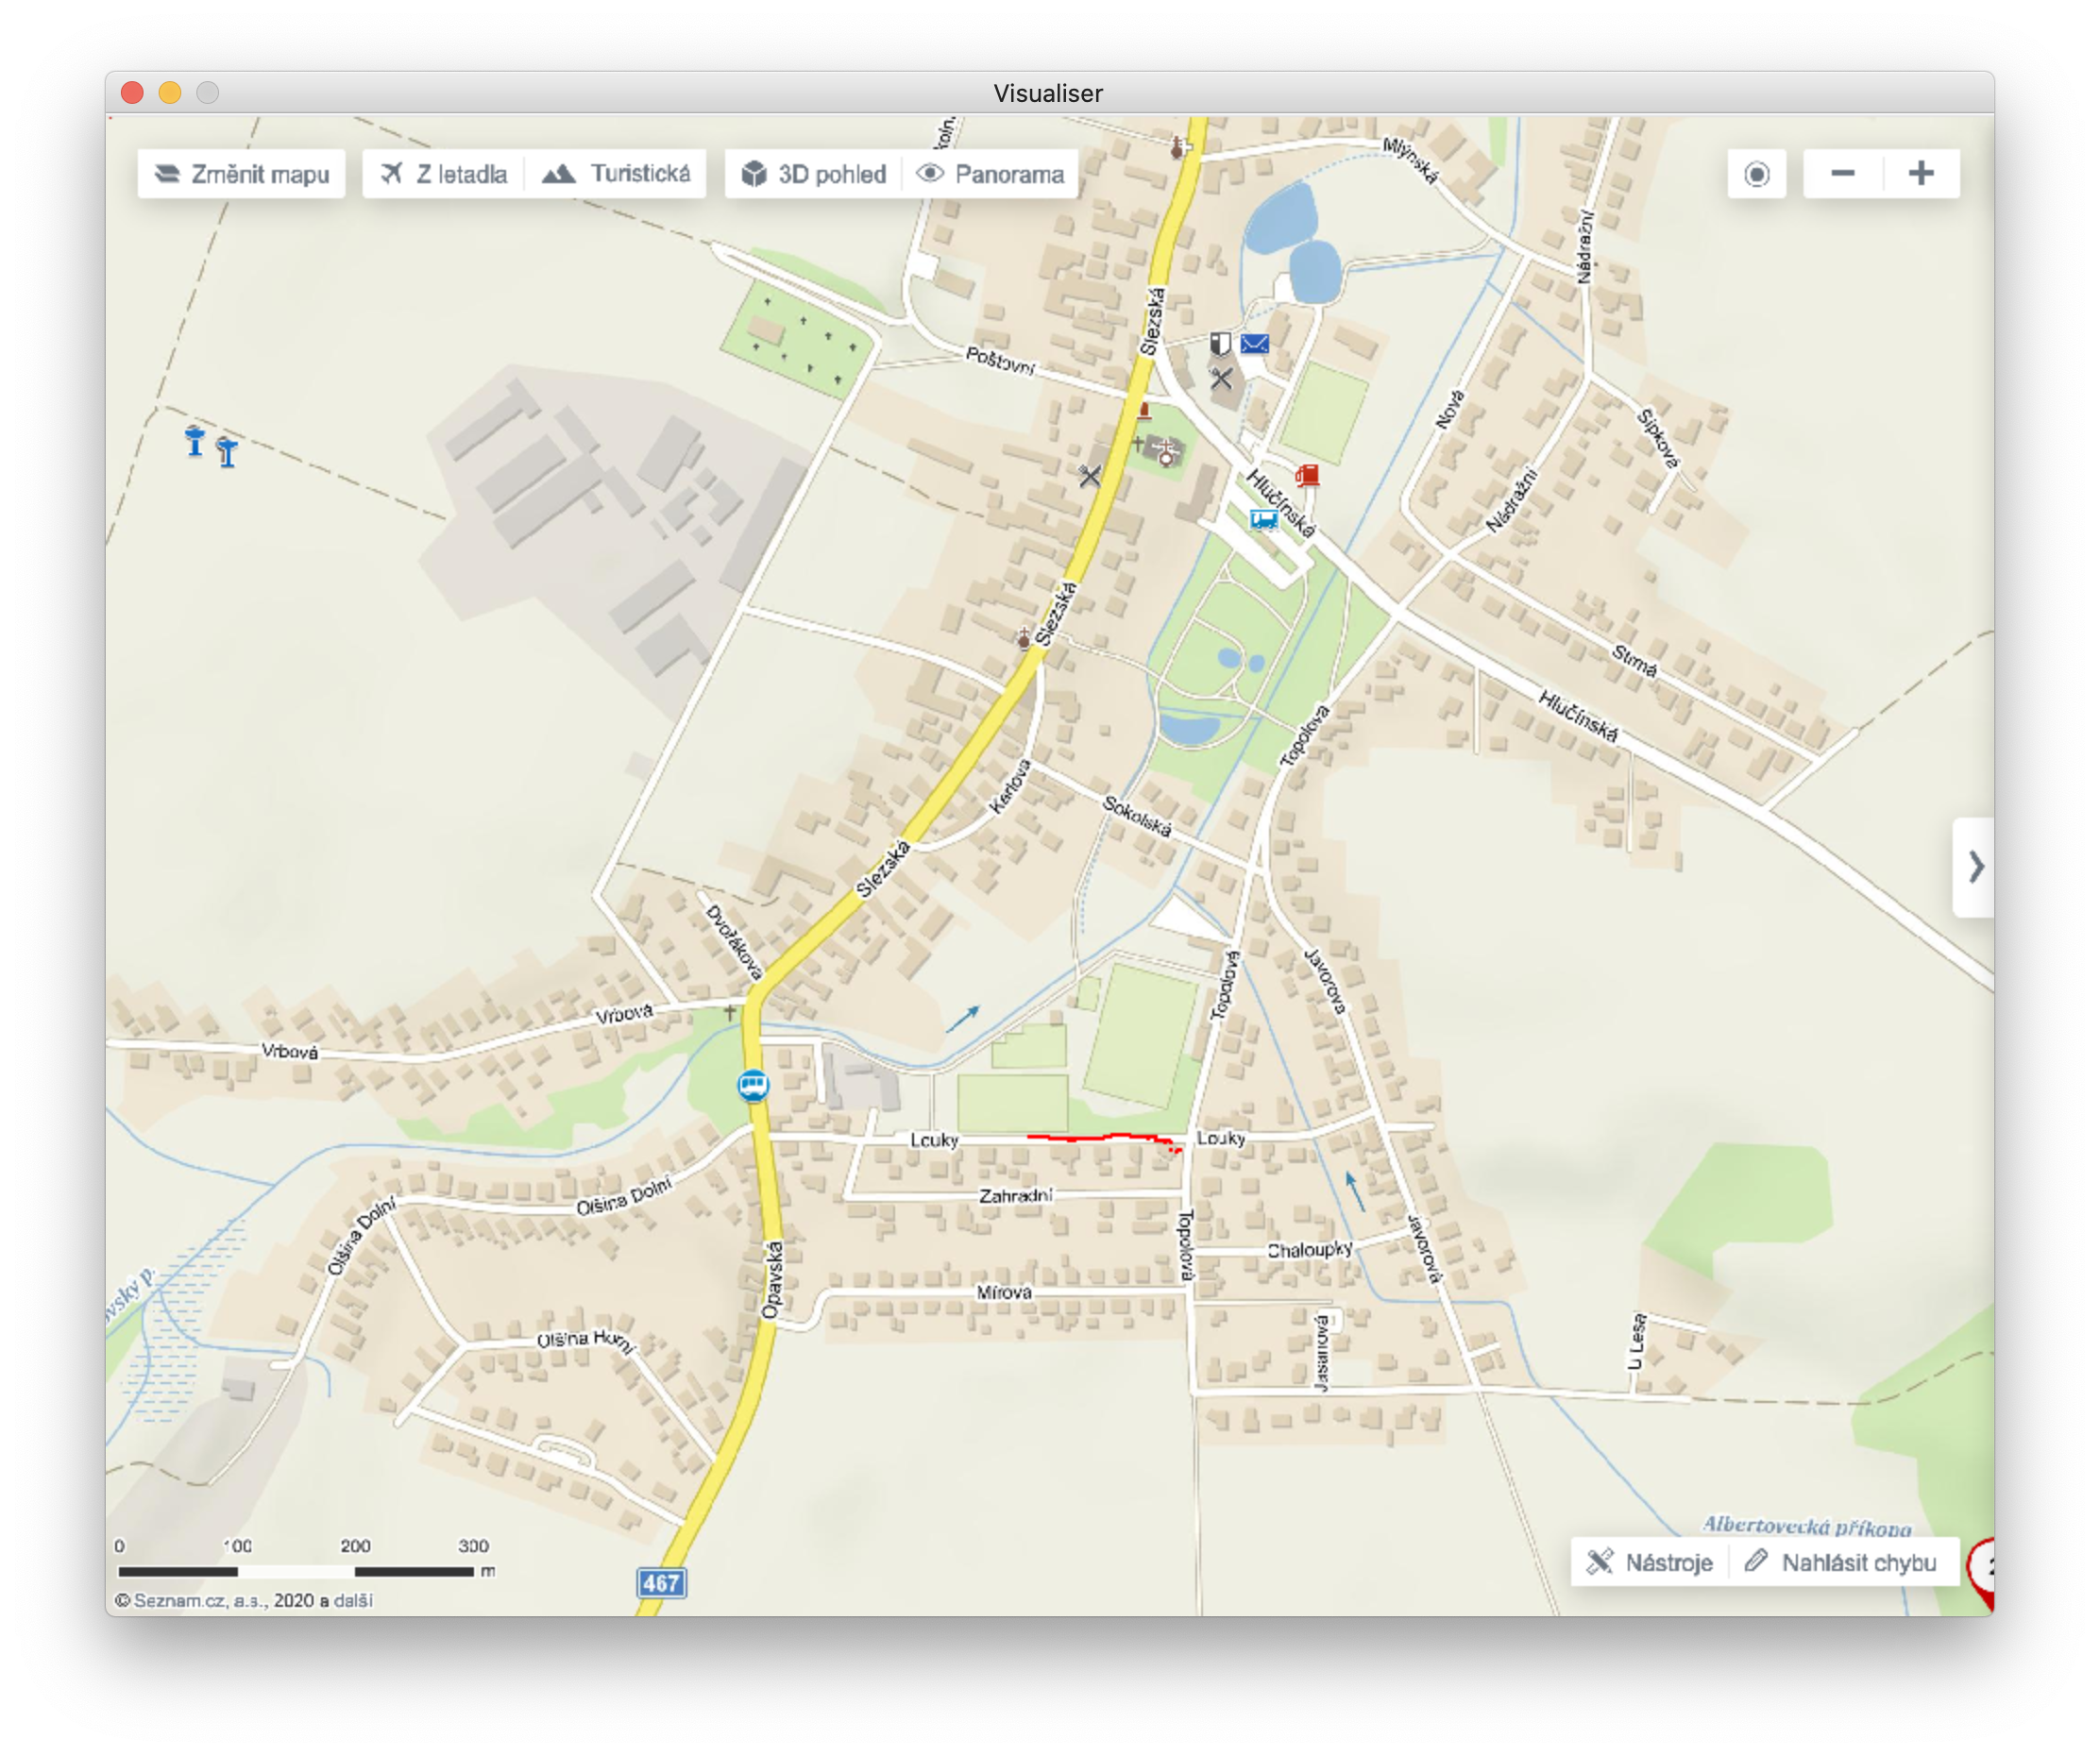
\includegraphics[width=0.9\textwidth]{Figures/louky.png}
    \caption{Rovná cesta středem ulice zaznamenaná pomocí GPS}
    \label{fig:louky}
\end{figure}

Jako další zajímavé měření lze považovat měření za jízdy osobním automobilem. Vozidlo dosahovalo rychlosti 30 km/h, tedy maximální
povolené rychlosti na silnici, na níž bylo měření prováděno. Měření bylo samozřejmě provedeno dvěma osobami, z níž
jedna řídila vozidlo, zatímco druhá operovala mobilní telefon s aplikací. Nedošlo tak k žádnému ohrožení bezpečnosti provozu.
Výsledek měření lze vidět na obrázku \ref{fig:olsinaautem}.

Na obrázku \ref{fig:olsinaautem} je vidět, že při vyšší rychlosti již naměřené hodnoty nejsou spojité. Stále se však objevuje
určitá odchylka, tentokrát ovšem skoro konstantní. Lze odečíst, že směr a rychlost vozidla není velký problém vyhodnotit při
vyšších rychlostech, kdy je projev odchylky relativně ke skutečné změně nízký. Ovládací software však vzniká za účelem řízení
autonomní platformy menších rozměrů kampusem univerzity. V takovémto případě je rychlost 30 km/h nereálná. Pro~vozidlo a jeho
náklad nemusí být vhodná a pro bezpečnost provozu v areálu je příliš vysoká. Dále si lze povšimnout, že ačkoliv je odchylka
přijatelně nízká pro určení směru pohybu, přesně určit pozici vozidla není možné. GPS modul velmi často umístil osobní automobil
do některého z domů stojících podél silnice. I přes takto vysokou odchylku lze jednoduše určit, po které silnici se vozidlo
momentálně pohybuje. Za účelem přesné navigace pouze pomocí GPS, což byl původní cíl výzkumu, je ovšem třeba přinejhorším
centimetrové přesnosti, jež GPS momentálně dosáhnout nedokáže.

\begin{figure}
    \centering
    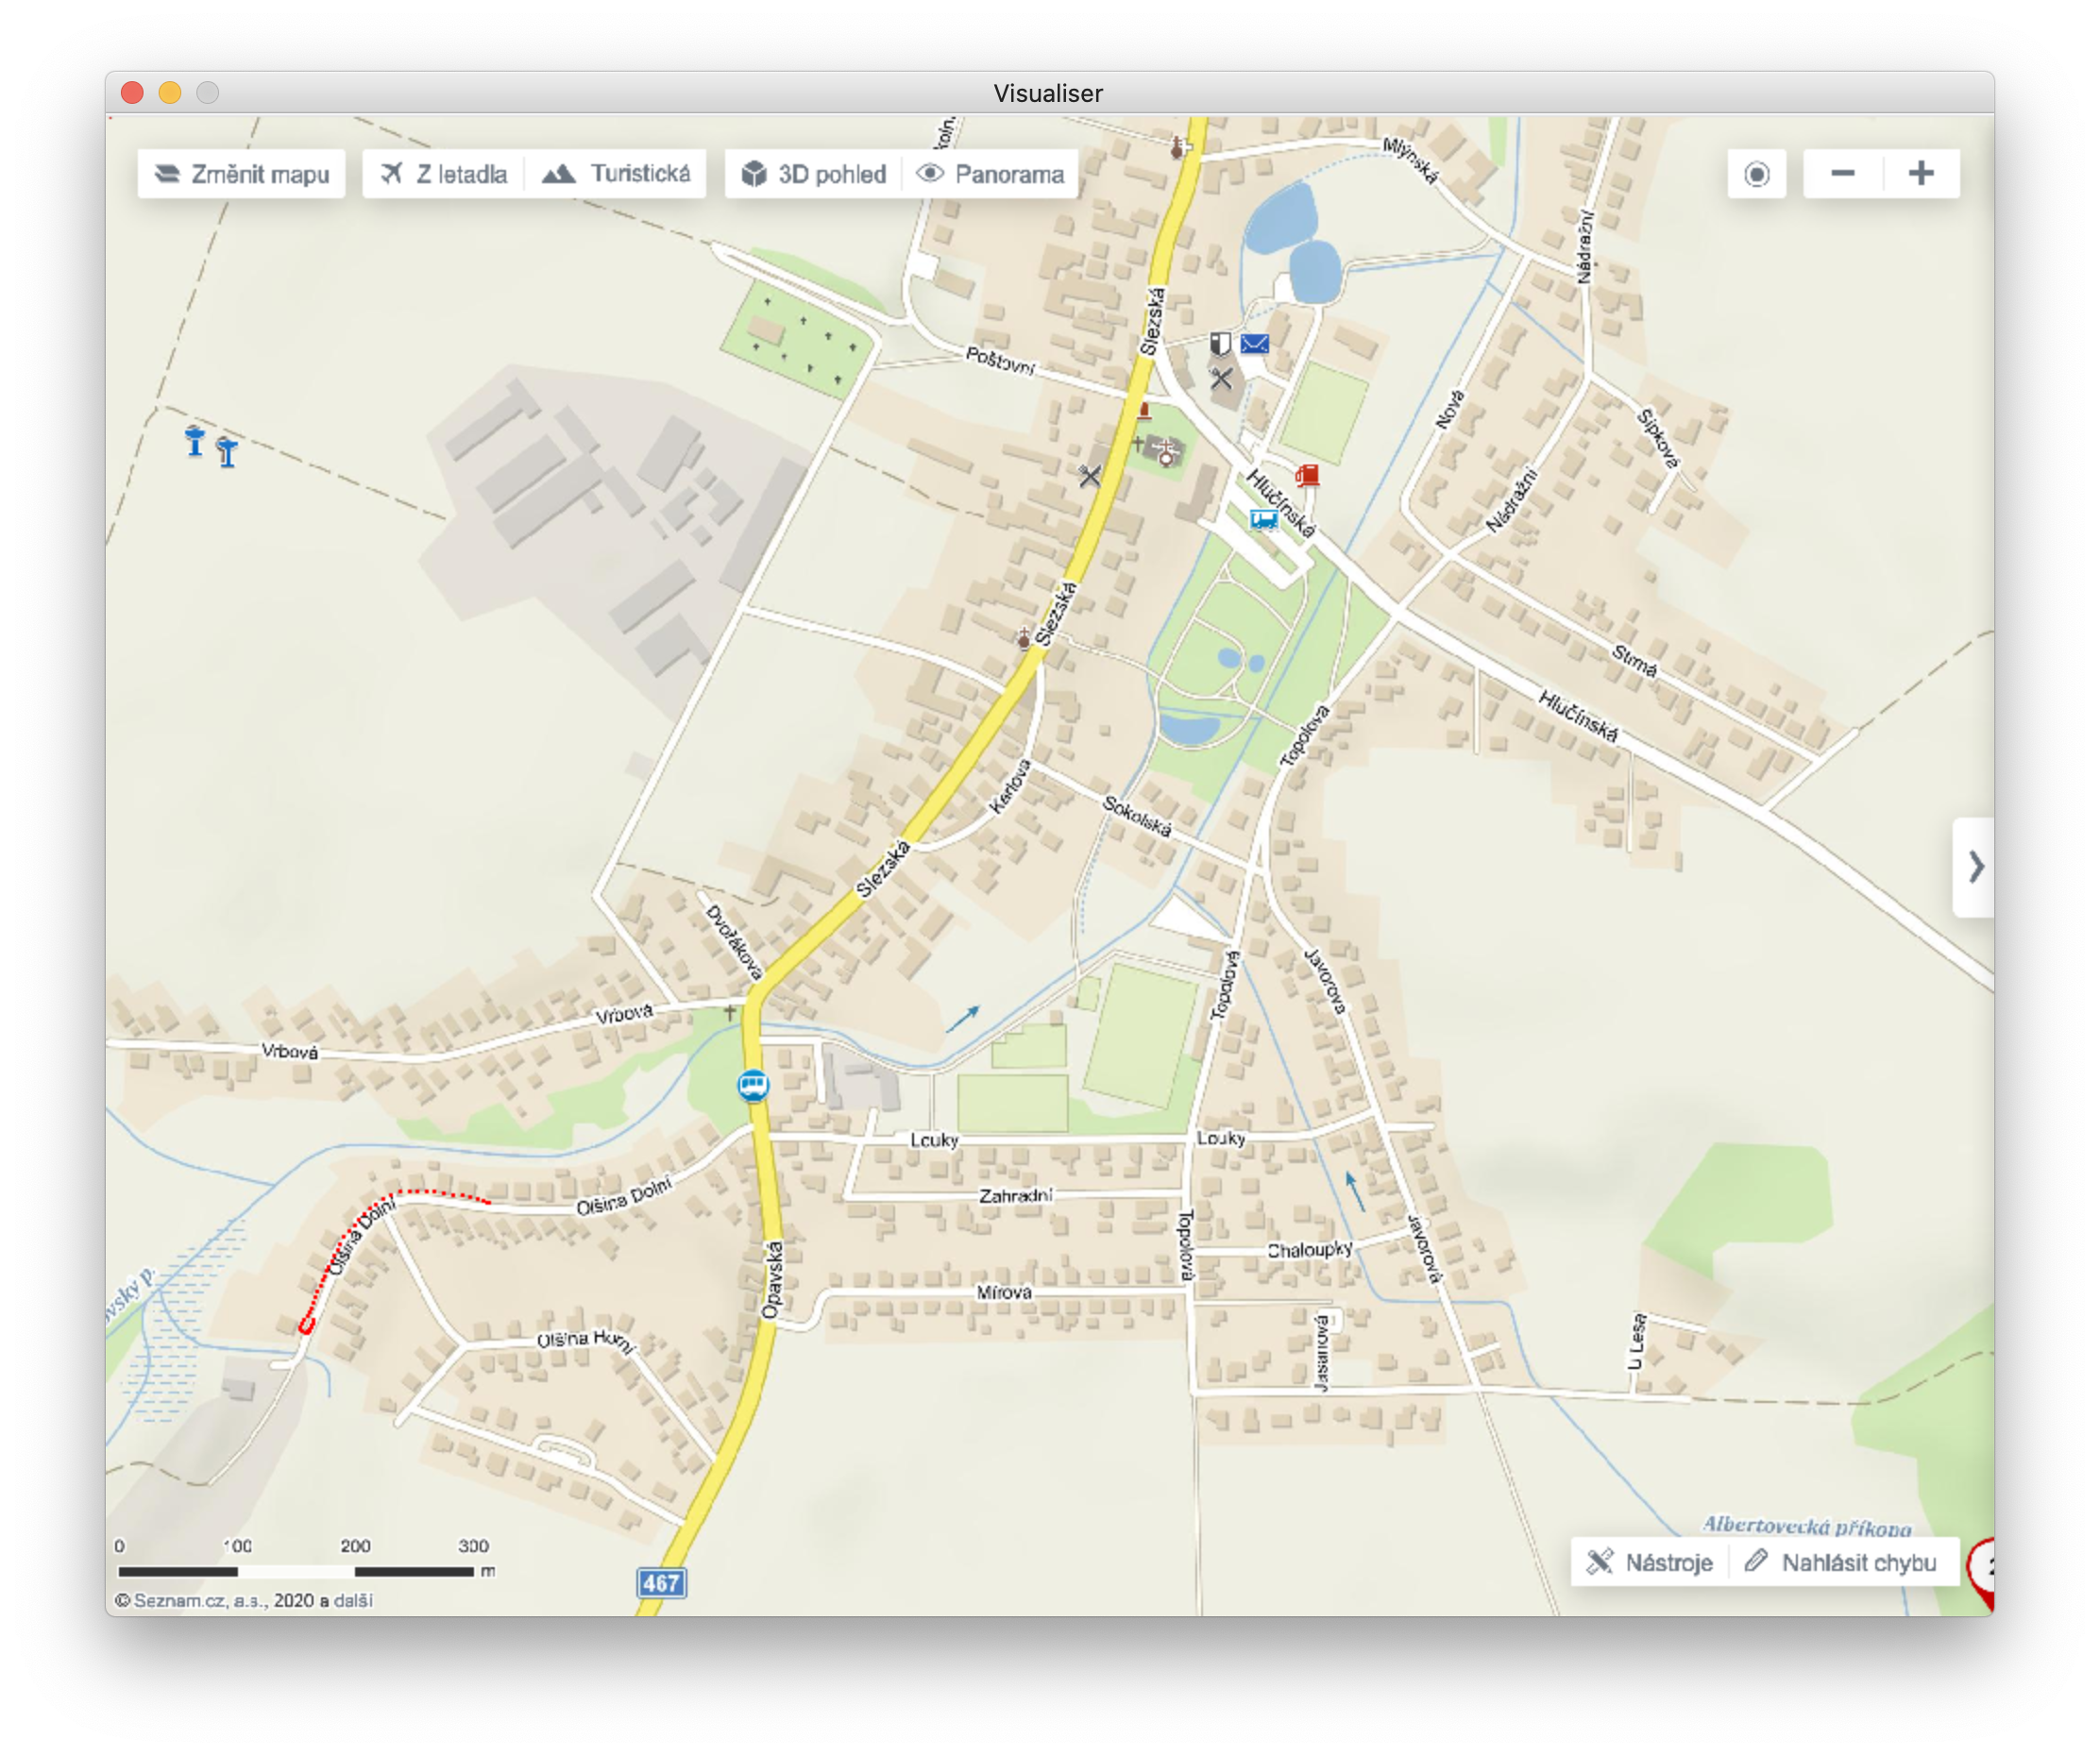
\includegraphics[width=0.9\textwidth]{Figures/olsinaautem.png}
    \caption{Krátká jízda osobním automobilem zaznamenaná pomocí GPS}
    \label{fig:olsinaautem}
\end{figure}

Výsledky všech měření v plné velikosti jsou obsaženy v příloze publikace.

\subsubsection{Návrhy řešení nepřesnosti GPS}

Ve snaze vytvořit funkční řízení čistě pomocí vstupu z GPS padlo v týmu zabývajícím se vývojem vozidla několik návrhů, jak danou
situaci vyřešit a odchylku odfiltrovat.

Jedním z návrhů bylo vzít nejbližší bod na na nejbližší silnici vzhledem k naměřené pozici, a~předpokládat, že se autonomní
platforma po dané silnici pohybuje. Tento návrh byl rychle zavrhnut. Pokud by se vozidlo pohybovalo po trajektorii neparalelní
se středem silnice, velmi rychle by opustilo silnici, ačkoliv by upravené hodnoty vykazovaly rovný pohyb po nadefinované cestě.

Druhým ze zavrhnutých návrhů byl návrh naměřenou hodnotu validovat výpočtem. Pokud vozidlo popojíždí určitou rychlostí s určitým
úhlem natočení kol, není reálné, aby náhle rychle změnilo svůj směr a začalo se pohybovat na opačnou stranu. Tato úvaha na první
pohled působí logickým dojmem, má ovšem jeden veliký problém. Abychom mohli validovat novou pozici na základě pozice předchozí
a dopočítané očekávané změny pozice, museli bychom si být jistí přesností pozice předchozí. Díky nepřesnosti GPS touto jistotou
ovšem nedisponujeme, a validace tak může být problematická a nepřesná.

Mezi návrhy se zařadilo také řešení hrubou silou -- využití většího množství GPS modulů a práce s průměrem naměřených hodnot.
Tento návrh však také nebyl bezchybný. Pokud by nebyly moduly synchronizovány a neaktualizovaly by své naměřené hodnoty všechny
najednou v krátkém časovém rozmezí, nemusel by průměr být vypovídající, zejména díky využití starých hodnot. Dále toto řešení
samozřejmě vyžaduje připojení většího množství GPS modulů k jednomu zařízení Raspberry~Pi. Nakonec však nedošlo k testování tohoto
řešení, neboť řízení čistě pomocí vstupů z GPS bylo ještě před testováním zavrhnuto.

\subsection{Pomalá odezva GPS} \label{gps-low-polling-rate}

Nepopiratelným problémem při snaze řízení vozidla pouze za pomocí GPS byla samozřejmě také pomalá odezva GPS modulu. GPS modul
aktualizoval souřadnice frekvencí pouze 1 Hz. Jedna aktualizace za sekundu pravděpodobně není žádný problém, pokud vozidlo řídí
člověk. Jedna aktualizace za sekundu by nepředstavovala problém ani při řízení pomocí vstupu z kamery. Pokud však má být vozidlo
řízeno pouze vstupem z GPS, je frekvence jednoho hertze příliš nízká. Jestliže vezmeme v~potaz, že se vozidlo může pohybovat
rychlostí několika metrů za vteřinu, zvláště poté v kombinaci s nepřesnou GPS, která může naměřit lokaci s odchylkou více než
jeden metr, mohlo by v praxi jednoduše dojít k situaci, kdy vozidlo například projede křižovatkou, na které mělo odbočit, nebo
křižovatku detekuje příliš pozdě, pokusí se zatočit, ale narazí například na obrubník, který díky absenci vstupu z kamery nebo
Lidaru v uvažovaném způsobu ovládání nedokáže detekovat.

Problém s rychlostí odezvy GPS je samozřejmě řešitelný investicí do GPS modulu s vyšší obnovovací frekvencí. V tomto momentě ovšem
bylo jasné, že řízení vozidla pouze pomocí GPS je v~nejlepším případě velmi nepraktické, v nejhorším případě velmi nebezpečné
pro vozidlo i okolí. O~nefunkčnosti tohoto řešení již nebylo třeba diskutovat, ovládání vozidla musí být implementováno jiným
způsobem. Proto tento problém zůstal neřešen.

\subsection{Směr natočení vozidla} \label{directions-and-angles}

Pro úspěšnou navigaci v prostoru je samozřejmě také nutné vědět, kterým směrem je vozidlo natočeno a kterým směrem se pohybuje.

Na platformě ovšem nebyl umístěn kompas. Proto bylo třeba improvizovat. Řídící kód musel tedy být znovu upraven, tentokrát takovým
způsobem, aby směr, kterým se vozidlo pohybuje, byl určován podle změny v naměřených GPS souřadnicích.

Zde ovšem vyvstal nový problém, vycházející z nedokonalosti a nepřesnosti GPS. GPS nedokáže zaměřit pozici se 100\% přesností,
vždy dojde k naměření s určitou odchylkou, která musí být při práci s naměřenými souřadnicemi započítána. Tato odchylka může
vozidlo na mapě umístit jinam, než kde ve skutečnosti je. Při vysokých rychlostech, kdy dochází k velkým změnám souřadnic,
je~odchylka relativně k absolutní změně zanedbatelná a odchylka mezi reálným a vypočítaným směrem pohybu dosahuje pouze
zanedbatelných hodnot. Vozidlo, jež je subjektem této práce, ovšem dosahuje pouze relativně nízkých rychlostí, převážně kvůli
bezpečnosti provozu. V nízkých rychlostech, ve~kterých absolutní změna pozice dosahuje nízkých hodnot, je odchylka způsobená
nepřesností GPS relativně o hodně vyšší, již není zanedbatelná, a odchylka mezi reálným a vypočítaným směrem pohybu je~schopná
dosahovat hodnoty až $180^{\circ}$. Hodnoty s tak vysokými odchylkami jsou samozřejmě v~praxi nevyužitelné. Problematice
nepřesnosti GPS se podrobněji věnuje sekce \filipref{gps-inaccuracy}.

Dalším problémem, který s sebou tento přístup určení směru přinesl, byla nemožnost určit směr natočení vozidla, když se vozidlo
nehýbalo. Tento problém měl nežádoucí projevy zejména po startu vozidla, kdy nebylo možné určit, kterým směrem musí platforma jet,
aby dosáhla cíle, a zda potřebuje zatáčet. V průběhu jízdy lze tento problém samozřejmě odstranit pamatováním si posledního
naměřeného směru před případným dočasným zastavením vozidla. Problém byl řešen obyčejným rozjetím autonomní platformy rovně
dopředu. Z naměřeného pohybu byl dopočten směr, a teprve poté došlo k umožnění zatáčení v řídícím softwaru.

Samotný výpočet směru pohybu vozidla je velmi jednoduchý. Za pomocí naměřených GPS souřadnic zjistíme, jaký pohyb vozidlo
vykonalo. Z předchozí a nově naměřené hodnoty vyčteme rozdíl v zeměpisné šířce i délce. Pomocí knihovny \emph{geopy} převedeme
rozdíl uvedený v zeměpisné šířce a délce na metry, a převedeme tak globální světové souřadnice na souřadnice kartézské. To nám
umožní využít goniometrické funkce a zjednoduššit výpočty, viz sekce \filipref{cartesian-coordinates}. Dále za~využití Pythagorovy
věty vypočteme celkovou vzdálenost, jakou vozidlo překonalo. Tímto získáme pravoúhlý trojúhelník, jehož přepona je dráha
pohybu vozidla, odvěsny poté reprezentují rozdíly v zeměpisné šířce a v zeměpisné délce. Následně stačí rozdíl v zeměpisné šířce
uvedený v~metrech vydělit celkovou vzdáleností. Touto operací získáme kosinus úhlu. Na získaný kosinus aplikujeme funkci arkus
kosinus, tedy funkci kosinu inverzní, čímž získáme úhel v rozsahu prvního a druhého kvadrantu. Jelikož však úhel může patřit do
třetího nebo čtvrtého kvadrantu kruhu, je třeba zkontrolovat, jestli je vozidlo pohybovalo směrem na západ. Jestliže je nová
lokalita vozidla západněji, provedla autonomní platforma pohyb vlevo v kartézských souřadnicích. V takovém případě pouze stačí
odečíst vypočítaný úhel od úhlu $360^{\circ}$. Tak získáme směr, kterým se v kartézských souřadnicích vozidlo pohybuje a zároveň
kterým směrem je momentálně natočeno.

Výpočet požadovaného směru pohybu je analogický, pouze se při výpočtu využije aktuální pozice vozidla a souřadnice waypointu.

Na základě vypočtených směrů je poté vypočítáno natočení kol, aby autonomní platforma svým pohybem mířila k cílovému waypointu.
Výpočet požadovaného natočení kol není vůbec složitý, jakmile známe směr, kterým se vozidlo momentálně pohybuje, a směr, kterým
by se vozidlo mělo pohybovat, aby dosáhlo svého cíle. Prostým odečtením těchto směrů od sebe získáme odchylku mezi požadovaným
a aktuálním směrem pohybu. Natočení kol následně může mít vůči rozdílu směrů lineární závislost, případně lze nastavit krokové
změny při určitých hodnotách odchylky.

\subsection{Práce s 2D prostorem} \label{cartesian-coordinates}

Jak již bylo předestřeno dříve, v této práci se často převádí geografické souřadnice na souřadnice kartézské. Díky elipsoidní
nátuře tvaru planety Země totiž nemusí jeden stupeň zeměpisné šířky odpovídat jednomu stupni zeměpisné délky relativně
k vzdálenosti. Navíc mezi vzdáleností vyjadřovanou jedním stupněm zeměpisné šířky a jedním stupněm zeměpisné délky neexistuje
univerzální poměr, neboť se poměr mezi těmito hodnotami mění na základě aktuální zeměpisné šířky.

Samozřejmě univerzitní kampus, pro který je autonomní platforma stavěna, není rozlohou nijak veliký, proto se nabízela možnost
pracovat s geografickými souřadnicemi jako by byly ekvivalentní souřadnicím kartézským, a předpokládat, že chyba způsobená tímto
zjednodušením bude zanedbatelná. Problémy s touto doměnkou ovšem byly odhaleny velmi rychle. Velikost chyby často přesahovala
rozumné hodnoty. Projev chyby bylo možné zachytit nejen při testování softwaru, ale~také při pouhém umístění vlastních značek
v libovolné veřejné mapové službě (při práci na projektu byly využívány služby OpenStreetMap a Mapy.cz). Samozřejmě bude umístění
značek opticky zkreslené, protože kreslíme na 2D projekci sférické planety. Toto zkreslení vytváří optickou chybu, jež nebude mít
na samotné výpočty vliv, i tak lze ale velmi dobře vidět nepřesnost námi využitého zjednodušení. Při umístění bodů na mapu tak,
aby hodnoty geografických souřadnic tvořily čtverec v~souřadnicích kartézských, tedy dva sousedící body mají vždy jednu souřadnici
stejnou, a rozdíl lišící se geografické souřadnice byl pro všechny čtyři strany stejný. Již na první pohled lze vidět, že~body
tvoří lichoběžník, ne čtverec, ačkoliv je lichoběžník také velmi zkreslený právě projekcí glóbu do 2D prostoru.

Po odhalení nepřesnosti tohoto zjednodušení bylo tedy rozhodnuto, že bude vyzkoušen jiný způsob zjednodušení výpočtů. Ačkoliv by
totiž správná práce s geografickými souřadnice elipsoidní planety byla nejpřesnější, pro relativně malý univerzitní kampus, který
lze navíc v řídícím softwaru považovat za 2D plochu, je implementace tohoto řešení zbytečně časově náročná s ohledem na~relativně
nízký benefit v daném měřítku. Proto momentální verze softwaru převádí geografické souřadnice na lokální kartézský systém. Tento
systém se prokázal jako dostatečně přesný v měřítku kampusu Vysoké školy báňské, a ačkoliv samozřejmě není přesný a přináší
s sebou také určitou chybu, díky využití lokálního kartézského systému je chyba dostatečně nízká.

Převod do lokálního souřadnicového systému je řešen způsobem předestřeným dříve v sekci \filipref{directions-and-angles}. Dva
geografické body se považují za úhlopříčku obdélníku. Délky stran obdélníku vypočteme aplikací funkce
\emph{geopy.distance.distance}. Dva body obdélníku již samozřejmě známe, zbylé dva body získáme tak, že vezmeme zeměpisné šířky
známých bodů, a zkombinujeme je se zeměpisnými délkami opačného bodu.

Vypočítané délky stran nám tak definují vektor, jenž odpovídá úhlopříčce obdélníku. Následně využijeme faktu, že obdélník lze
definovat také kombinací bodu a vektoru. Jeden vrchol obdélníku umístíme do bodu (0, 0). Když k tomuto bodu poté přičteme
vypočtený vektor, získáme opačný vrchol. Tyto vrcholy nám nyní reprezentují geografické souřadnice v lokálním kartézském systému.

Délku úhlopříčky samozřejmě můžeme spočítat buď aplikací Pythagorovy věty, nebo funkcí \emph{geopy.distance.distance}. Využití
zmíněné funkce z knihovny \emph{geopy} bude pravděpodobně přesnější, Pythagorovu větu ovšem naopak můžeme aplikovat i v případě,
kdy neznáme původní geografické body, které byly převedeny do kartézského souřadnicového systému. Takový případ může nastat třeba
po zavolání funkce, jež jako své argumenty přijímá pouze kartézské souřadnice. Zdrojový kód funkce, ale ani funkce nebo metody
touto funkcí volané, již k původním geografickým souřadnicím nemají jak přistoupit.

Nespornou výhodou kartézského souřadnicového systému je jednoduchost jeho využití. V kartézském souřadnicovém systému lze také
bez jakýchkoliv problémů aplikovat funkce sinus a kosinus, které jsou samozřejmě kritické při práci s úhly. Dále na počtech
s kartézskými souřadnicemi často není nic složitého. Díky jejich přímočarosti tak zdrojový kód zůstává jednoduchý, čitelný,
vývoj je~rychlejší a také je sníženo riziko výskytu chyb.

Při navigaci vozidla, a zejména při práci s mapovými podklady, je univerzitní kampus považován za 2D plochu. Areál možná nelze
považovat za vodorovný, zároveň jej ale nikdo nemůže nazvat kopcovitým, nebo dokonce hornatým. Výškové rozdíly napříč areálem jsou
dostatečně nízké, aby se daly považovat za zanedbatelné. Při navigaci tedy není třeba plánovat cestu tak, aby vozidlo nemuselo
podstupovat dlouhé stoupání do kopce a zbytečně plýtvat energií. Občasné krátké stoupání pak může způsobit zpomalení pohybu
vozidla, za takovým účelem je ale na ovládacím serveru běžícím na~autonomní platformě samotné implementován PI regulátor, který
právě v takovémto případě zaznamenaný pokles rychlosti vykompenzuje zvýšením kroutivého momentu elektromotoru, aby udržel rychlost
na požadované hodnotě. PI regulace je probrána v sekci \filipref{pi-controller}.

\section{Řízení vozidla pomocí detekce grafických kódu}

Narozdíl od řízení pomocí GPS dopadly pokusy o prototyp řízení za využití detekce grafických kódů úspěšněji. Obyčejné následování
grafického kódu bylo s rozumnou přesností a úspěšností zprovozněno již při prvním testování na fyzickém vozidle. I přes relativní
úspěch testování má však toto řešení také své úskalí, pramenící především z jednoduchosti řešení, proto není tento způsob řízení
v praxi používán. Přesto výzkum a testování tohoto řešení, podobně jako v případě řízení pomocí GPS, přineslo nejen řadu poznatků,
ale také technické zázemí a využitelný zdrojový kód.

\subsection{Implementace řízení}

Při implementaci tohoto druhu řízení byla na vozidlo upevněna obyčejná webkamera. Vstup z webkamery analyzoval program nezávislý
na řídícím softwaru, který je subjektem této práce. Analyzační software společně s kamerou byly kalibrovány na určitou velikost
grafického kódu. Po správné kalibraci dokázal software správně určit vzdálenost kódu od vozidla na základě jeho nakonfigurovaných
rozměrů. Dále dokázal software spočítat také vzdálenost od středu obrazu. Tato hodnota byla následně využita pro výpočet natočení
kol vozidla. Software pro analýzu obrazu ovšem není předmětem této práce a byl vyvíjen jiným členem výzkumného týmu.

Software analyzující vstup z kamery také implementoval obyčejný TCP server, jež na požádání vrátil údaje odečtené ze vstupu
z webkamery. Ve své odpovědi vrací server vzdálenost detekovaného kódu od vozidla a vzdálenost detekovaného kódu od středu obrazu.
Řídící software si opakovaně o tyto hodnoty žádá a na jejich základě počítá odchylku mezi směrem, kterým vozidlo momentálně
směřuje, a úhlem, pod kterým na grafický kód nahlíží. Natočení kol je následně nastaveno na hodnotu této odchylky, nejvýše však
$20^{\circ}$, tedy maximální úhel natočení přední soupravy, aby autonomní platforma vždy směřovala nejkratší cestou k detekovanému
kódu. Aby nedošlo ke kolizi mezi vozidlem a objektem, na kterém je upevněn grafický kód, je software naprogramován tak, aby
vozidlo zastavil v momentě, kdy je detekovaná vzdálenost kódu menší nebo rovna dvěma metrům.

K výpočtu odchylky je třeba pouze matematika základní školy. Představíme si trojúhelník, jehož tři vrcholy jsou objektiv kamery,
střed projekce, a grafický kód. V takovém trojúhelníku bude přeponu představovat úsečka mezi objektivem kamery a grafickým bodem.
Odchylku samotnou představuje úhel mezi přeponou a úsečkou spojující střed projekce. Délku této strany trojúhelníku neznáme, známe
ovšem délky zbylých dvou stran, a víme, že je daný trojúhelník pravoúhlý. Pro~výpočet úhlu tedy můžeme využít poměr přepony ku
protilehlé straně. Délkou protilehlé strany je zde vzdálenost bodu od středu projekce, délkou přepony je vzdálenost bodu
od vozidla. Samotný poměr nám představuje sinus hledaného úhlu. Na poměr tedy aplikujeme funkci arkus sinus, funkci inverzní k
funkci sinus, a získáme hledanou odchylku.

\subsection{Výsledek testování}

Řešení se při testování projevilo jako funkční, ovšem omezené a v praxi hůře použitelné. Jako hlavní problém samozřejmě vyvstává
absence analýzy okolí vozidla. Stejně jako při řízení pomocí GPS, i~zde si vozidlo není vědomo svého okolí. Mohlo by tak snadno
dojít k situaci, kdy autonomní platforma například narazí do jednoho z řady prémiových vozů německých značek, které jejich
majitelé rádi parkovali v místech, kde často docházelo k testování nehotového softwaru pro autonomní řízení, nebo, v horším
případě, ohrozí zdraví lidí náhodou se pohybujících okolo vozidla. Pokud by mělo dojít k reálnému využití takto řízeného vozidla,
analýza okolního prostředí samozřejmě bude nezbytná. Je však třeba zmínit, že v případě testování se jednalo teprve o první
prototyp, jenž měl sloužit k vyzkoušení daného způsobu řízení. Cílem při prvním testování samozřejmě nebylo, a ani nemohlo být,
vytvořit na první pokus dokonalý systém.

Jako druhý, a z hlediska využití vozidla také podstatně závažnější, problém se nabízí omezená flexibilita řešení. Zatímco při
řízení pomocí GPS stačí pro změnu cesty autonomní platformy pouze nadefinovat jinak waypointy, případně aktualizovat digitální
mapové podklady, v případě řízení pomocí grafických kódu je třeba fyzicky rozmístit grafické kódy tak, aby software vždy věděl,
kde má v aktuální situaci platformu směřovat. Grafické kódy musí být vidět, nesmí být například blokovány zaparkovaným vozem,
poničené okolo jdoucí osobou se špatnými úmysly, poničené vlivem počasí, apod. Dále lze tímto způsobem nadefinovat pouze jednu
cestu, aby software vždy dokázal jednoduše deterministicky rozhodnout o správné cestě. Posledním projevem neflexibility daného
způsobu řešení je také nutnost fyzicky přesunout grafické kódy při každé změně plánované cesty.

Za problém lze považovat také fakt, že vozidlo při detekci kamery směřuje přímo k nejbližšímu kódu. Kódy samozřejmě musí být
rozmístěny mimo silnici či chodník, aby neblokovaly cestu. Ovšem kódy umístěné mimo silnici dokážou vozidlo svést z cesty
v lepším případě pouze na trávník, v~horším případě jej navedou přímo do nečekané překážky. Tento problém však je řešitelný,
například vynucením určitého odstupu od kódu a udržování kódu v určité vzdálenosti od boku vozidla.  V~tomto případě by ale musely
všechny kódy být umístěny pouze po jedné straně vozidla. Druhým možným řešením je převod detekovaného grafického kódu na waypoint
na mapě. Toto řešení ovšem vyžaduje využití mapových podkladů a vstupů z GPS pro řízení platformy, a zabíhá již do~podkapitoly
\filipref{combination-of-driving-inputs}

\subsection{Možné využití v praxi}

I přes určitá omezení tohoto způsobu řízení ovšem není možné daný způsob prohlásit za nepoužitelný. Ačkoliv je nevhodný
při navigaci kampusem pomocí předem neznámé trasy, může skvěle posloužit například pro přesné zaparkování vozidla po dosažení
cíle. K parkování lze samozřejmě využít například horizontální značení parkovacího místa. Očekává se ovšem, že autonomní platforma
bude objíždět velké množství budov spadajících pod kampus Vysoké školy báňské. V takovém případě ovšem nemusí jít vždy zaparkovat,
například z důvodu obsazenosti parkovacích míst, nebo z důvodu velké vzdálenosti nejbližšího parkovacího místa od budovy. Toto by
mohlo způsobit problémy třeba při případné implementaci automatizovaného nakládání a vykládání vozidla. Navíc možnost vytvářet
nová parkovací místa rezervovaná pouze pro autonomní výzkumná vozidla nevyniká svou praktičností, už jen díky nutnosti vytvoření
nového horizontálního značení.

Jako alternativa se v takovéto situaci nabízí právě využití grafického kódu, který stačí pouze vytisknout ve správné velikosti
a umístit na vertikální plochu. Vozidlo by po detekování kódu mohlo přesně zaparkovat v předdefinované vzdálenosti od kódu. Takto
by bylo možné přesně a relativně jednoduše dovést vozidlo až do přesně určené finální pozice. Tato funkcionalita dokáže umožnit
nejen dříve zmíněné robotizované nakládání a vykládání autonomní platformy, jež má sloužit k rozvozu materiálu napříč kampusem,
ale také přesné zaparkování v garáži nebo jiných vnitřních prostorech, ve kterých samozřejmě nelze využít technologii GPS.

\section{Řízení vozidla kombinací vstupů z GPS, kamery, a za využití mapových podkladů} \label{combination-of-driving-inputs}

Jasným výsledkem předchozího výzkumu tedy je nutnost implementace řízení za pomocí kombinace více vstupů. Tato implentace tak bude
kombinovat vyhledávání cesty pomocí mapových podkladů k nalezení správné cesty, a vstupy ze soustavy kamer a lidarů k zajištění
bezpečnosti provozu, vyhýbání se překážkám, udržování správné trajektorie, aby vozidlo např. odchylkou GPS nesjelo z~vozovky,
ale také k vyhledávání zatáček a křižovatek, na kterých poté pomocí mapových podkladů proběhne rozhodnutí o následujícím pohybu
autonomní platformy, aby bylo korektně dosaženo cíle. Cíl samozřejmě bude definován waypointy. Při vývoji bude využito nejen
poznatků, ale také kódu z předchozího výzkumu.

Bohužel, vývoj tohoto způsobu autonomního řízení je náročný a navazuje na předchozí výzkum, projekt bude vývoji ještě nějakou
dobu, a přesahuje rozsah této publikace. Navíc byla práce na~projektu autonomního řízení negativně ovlivněna pandemií koronaviru
SARS-CoV-2 \cite{pandemic-source} a stoupající cenou kryptoměn \cite{bitcoin-rally-source}. Pandemie koronaviru ztížila testování
vozidla a práci s fyzickým vozidlem vynucení práce z domova, způsobila silný nedostatek webkamer, které byly na projektu potřeba
kvůli snímání okolí, a kombinace vysokého zájmu těžařů o grafické karty, a snížené produkce grafických karet a počítačových čipů
obecně, znemožnila získání hardwaru potřebného pro implementaci plně autonomního řízení
\cite{bitcoin-miners-gpu-source,webcam-shortage-source}. Práce však bude do budoucna stále pokračovat, pravděpodobně poté bude
popsána v jiné publikaci.

\chapter{Práce s mapovými podklady} \label{osm-chapter}

Při práci s mapovými podklady jsou využity hned dvě mapové služby, Mapy.cz společnosti Seznam.cz, a.s., a komunitní mapový projekt
OpenStreetMap.

Mapy.cz jsou využívány především pro grafické podklady. Dále je využíváno API Mapy.cz pro~implementaci webové aplikace. Důvody
využití služby Mapy.cz souvisí především s extenzivním, avšak jednoduchým API, ale také s jejím českým původem. Vývojáři Mapy.cz
spolupracují přímo s~českými úřady a často tak dokážou zaznamenat změny v silniční síti rychleji než zahraniční nebo komunitní
mapové služby. Drobnou roli hraje také vlastenecký sentiment.

OpenStreetMap poté slouží jako poskytovatel veřejně dostupných vektorových mapových podkladů.

Při vývoji projektu byl věnován čas výběru správnému zdroji vektorových mapových podkladů. Mapy.cz působily jako primární kandidát
na zdroj podkladů, a to především díky svých již dříve zmíněných časnějších aktualizací na základě změn v silniční síti.
Při studování dokumentace API Mapy.cz byl však objeven znepokojující fakt -- Mapy.cz veřejně poskytují pouze grafické podklady.
Na dotaz, zda je možné využít vektorové podklady společnosti Seznam.cz, a.s., bylo odpovězeno, že~v~současné době jsou tyto
podklady používány pouze interně a existují pouze v binárním formátu. Společnost Seznam.cz, a.s. vyjádřila ochotu exportovat
a poskytnout svá data pro akademické účely, ovšem pro jednoduchost využití bylo rozhodnuto, že budou využity podklady poskytované
projektem OpenStreetMap.

\section{Stahování mapových podkladů a jejich zpracování}

Projekt OpenStreetMap, zvolený poskytovatel mapových podkladů, umožňuje data exportovat mimo jiné také ve formátu XML. Pro získání
souboru stačí vytvořit obyčejný HTTP GET požadavek a~požadovanou exportovanou oblast specifikovat v parametrech URL. Server
v odpovědi vrátí soubor s~mapovými podklady. Soubor lze takto jednoduše získat například pomocí programu \emph{curl}.

Pro stahování a export mapových podkladů byl vytvořen separátní skript implementován v~jazyce Python. Tento skript dokáže stáhnout
soubor s mapovými podklady, zpracovat jej, uložit zpracovaná data ve vlastním formátu, a následně smazat soubor s původními
mapovými podklady ve formátu XML.

Implementace separátního skriptu pro získání mapových podkladů s sebou přinásí určité množství výhod. Skript je možné periodicky
spouštět jako cronjob, ať už přímo v operačním systému, nebo například jako kontejner v Kubernetes. Dále je možné část zpracování
podkladů převést z~plánovacího softwaru do separátního programu, a tím zjednodušit logiku samotného plánovacího softwaru.
A nakonec, využití vlastního formátu pro uložení dat nám umožní jednoduššeji přidat do~souboru vlastní data a dodatečný kontext,
viz sekce \filipref{smarter-maps}.

K načtení textového XML souboru je využita knihovna \emph{osmium}. Z tohoto souboru jsou přečteny uzly a cesty. Relace jsou
ignorovány. Při zpracování cest jsou uloženy pouze cesty povolených typů, ostatní typy cest jsou ignorovány. Mezi ignorované typy
patří např. \emph{footway}, \emph{corridor}, \emph{steps}. Podklady OSM často obsahují například chodníky či chodby, je ovšem
velmi nežádoucí, aby se vozidlo pokoušelo projíždět například chodbou budovy. Po načtení všech cest jsou nakonec z mapových
podkladů odstraněny také uzly, ke kterým nevede žádná cesta. Uzly v reálném světě představují například křižovatky nebo spojení
chodeb. Ovšem v případě například vnitřního uzlu, tedy spojení chodeb v budově, není třeba uzel ukládat v paměti softwaru a dále
s ním pracovat, neboť chodby jsou již dříve z podkladů odstraněny a uzel by neměl reálné využití.

Zpracovaná data jsou dále skriptem naformátována a uložena ve formátu JSON. Po dokončení exportu je XML soubor smazán.

\section{Vyhledání nejbližší silnice na mapě}

Vyhledání nejbližší silnice je důležité nejen za účelem určení aktuální pozice vozidla na mapě, ale také při umisťování waypointů,
které se vždy umisťují na silnici, viz sekce \filipref{target-definition}. Autonomní platforma se samozřejmě pohybuje po silnici,
a plánovací software musí vědět, kde se vozidlo momentálně nachází i v momentě, kdy nepřesná GPS (viz sekce
\filipref{gps-inaccuracy}) umístí autonomní platformu mimo definovanou silnici. Dále samozřejmě musí plánovací software vědět,
na~které silnici se nachází daný waypoint, aby dokázal správně naplánovat cestu.

Cestu lze v mapových podkladech definovat dvěma způsoby. Počátečním a koncovým bodem, nebo bodem a vektorem určujícím směr a délku
cesty. Oba způsoby definice cesty jsou využity při~určování nejbližší silnice. Dále je uvažováno, že nejkratší cestou
z libovolného bodu k libovolné silnici je úsečka kolmá k dané silnici, pokud taková úsečka existuje. V opačném případě
je nejkratší cestou úsečka spojující daný bod s bližším koncem silnice.

Pro určení nejbližší silnice využijeme výpočet průsečíků dvou přímek \cite{line-line-intersection-source}.
Jako první přímku uvažujeme přímku definovanou počátkem a koncem silnice. K získání druhé přímky je následně třeba vzít normálový
vektor k vektoru definujícímu danou silnici. Získaný normálový vektor umístíme do~uvažovaného bodu, tedy například do aktuální
pozice vozidla nebo neupravené pozice uživatelem definovaného waypointu. Tímto získáme přímku kolmou k dříve získané přímce.
Následně na~získané přímky aplikujeme funkci výpočtu průsečíku přímek, a zkontrolujeme, zda se daný průsečík nachází zároveň
na úsečce představující silnici. Pokud ano, nejkratší cestu z uvažovaného bodu k~dané silnici definujeme jako úsečku z uvažovaného
bodu do průsečíku přímek. Pokud ne, nejkratší cesta bude cesta z daného bodu k bližšímu okrajovému bodu silnice. Tento algoritmus
následně stačí v cyklu aplikovat na všechny silnice definované v mapových podkladech, a takto nalézt silnici, ke které vede
nejkratší cesta. Tímto získáme nejen nejbližší silnici, ale také bod na dané silnici, ve~kterém se nachází vozidlo, nebo ve kterém
by měl být umístěn waypoint.

\section{Plánování cesty za využití mapových podkladů}

%TODO: BFS (nebo variace) nad cestami, rád bych naprogramoval, jestli nestihnu, okecat

\chapter{Webová aplikace} \label{web-app}

V kapitole \filipref{target-definition} bylo předestřeno využití webové aplikaci ke vzdálenému ovládání vozidla. V současné době
lze autonomní platformu ovládat pomocí vizualizéru, jenž je součástí plánovacího softwaru. Toto řešení je ovšem dočasné a slouží
především k ulehčení vývoje a zachytávání chyb. Při skutečném využití by bylo přinejlepším nepraktické. Využívání vizualizéru,
mimo své negativní dopady na nároky ovládacího softwaru díky nutnosti vykreslovat vozidlo na~mapu a vyobrazovat jeho pohyb,
znemožňuje kontejnerizaci softwaru pro plánování cesty a vynucuje spouštění ovládacího softwaru na zařízení, ze kterého chceme
autonomní platformu ovládat. Za další nevýhodu lze považovat nutnost instalace interpreteru jazyka Python na cílovém stroji, nebo
daný interpreter přibalit k distribuci plánovacího softwaru.

Webová aplikace je v dnešní době již víceméně standardním řešením, jež řeší všechny dříve zmíněné problémy. Software pro plánování
cesty vozidla může běžet nezávisle na uživatelském rozhraní v kontejnerizovaném prostředí a vystavovat své REST API
pod nakonfigurovaným portem. Backend webové aplikace může běžet na stejném stroji či clusteru, jako plánovací software, nebo může
být samozřejmě spuštěn kdekoliv jinde. Uživatel poté webovou aplikaci může využívat jednoduše za pomoci libovolného moderního
webového prohlížeče. Prohlížeč si od serveru vyžádá statické soubory a vykreslí webovou aplikaci, jež následně očekává vstup
od uživatele a zároveň graficky vyobrazuje aktuální informace o vozidlu. Uživateli tak stačí mít k dispozici libovolný stroj
s moderním prohlížečem. Není třeba instalace žádného softwaru, může být využito libovolné zařízení, logika plánování cesty
a logika grafického vyobrazování informací o vozidle je od sebe oddělená, a všechny potřebné aktualizace jsou proveditelné
na straně backendu.

\section{Implementace frontendu webové aplikace}

Volba technologií využitých na frontendu určitě nikoho nepřekvapí. Pro práci s mapovými podklady je využíváno API mapové služby
Mapy.cz (viz kapitola \filipref{osm-chapter}), jež umožňuje nejen vykreslování vozidla a waypointů, ale také registrovat interakce
s mapou a implementovat ovládání vozidla a vytváření waypointů. Webová stránka je definována značkovacím jazykem HTML a logika
webové aplikace je naprogramována v jazyce Javascript. Knihovna služby Mapy.cz je jediná závislost využitá v implementaci
frontendu webové aplikace, s její výjimkou je využit pouze čistý Javascript.

Frontend webové aplikace po svém načtení prohlížečem začne periodicky obnovovat aplikaci pomocí HTTP requestu na backend aplikace.
Po přijetí odpovědi serveru jsou automaticky aktualizovány mapové podklady.

Dále frontend definuje vytváření a mazání waypointů, jež definují cíl cesty vozidla.

Po kliknutí na mapu je poslán HTTP dotaz na API serveru. Server následně notifikuje plánovací software o uživatelově snaze
vytvořit waypoint. Software waypoint vytvoří a vloží jej na nejbližší cestu definovanou v mapových podkladech vozidla.
Po vytvoření waypointu je vynucena aktualizace mapových podkladů, aby se nově vytvořený waypoint promítl na mapě.

Kliknutím na waypoint je možné daný waypoint smazat. Mazání waypointu je provedeno způsobem analogickým k vytváření waypointu,
pouze je volán jiný endpoint backendu.

\section{Implementace backendu webové aplikace}

Volba technologií na backendu je již zajímavější, už jen z důvodu vyššího výběru technologií použitelných pro vývoj backendu.
Pro tvorbu serveru byl zvolen programovací jazyk Kotlin spárovaný s frameworkem \emph{Ktor}.

Jazyk Kotlin je moderní, objektově orientovaný jazyk s prvky funkcionálního programování. Jazyk Kotlin je tvořen firmou JetBrains
a je možné jej kompilovat pro více platform. Primárně je jazyk Kotlin kompilován pro platformu JVM, kde může využívat celého
ekosystému jazyka Java, dále však může být kompilován do nativního strojového kódu, nebo transpilován do jazyka Javascript. Jazyk
Kotlin v současné době slouží jako oficiální jazyk pro tvorbu aplikací mobilního operačního systému Android
\cite{kotlin-android-source}.

Framework \emph{Ktor} je technologie implementovaná v jazyce Kotlin, sloužící k implementaci asynchronních REST API. Samotné API
webové aplikace ovšem není vyvíjeno s důrazem na asynchronost, neboť požadavky na výkon rozhranní nikdy nebudou tak vysoké, aby
odůvodnily čas strávený implementací asynchronního programu.

Důvod volby těchto technologií byla snaha ukázat modularitu systému o více komponentách využívajících protokol HTTP
pro komunikaci, a možnost využití libovolné technologie a jazyka v~takto nadesignovaném systému. Pro uvažovanou aplikaci by
samozřejmě jazyk Python byl naprosto validní volba, v praxi je ovšem často vhodné využití většího množství jazyků a technologií,
především díky lišících se předností různých jazyků, nebo dostupnosti knihoven či frameworků pro daný jazyk nebo platformu. Druhým
důvodem volby jazyka Kotlin byla snaha vyzkoušet využití frameworku \emph{Ktor} v praxi.

Backend definuje REST API, jež, kromě vydávání statických souborů, implementuje endpointy analogické REST API softwaru
pro plánování cesty, popsaném v podkapitole \filipref{rest-api}. Rozdíl mezi API plánovacího softwaru, a API backendu webové
aplikace, je ve validaci prováděné daným API. API plánovacího softwaru, z důvodů jednoduchosti implementuje pouze minimální
validaci, nemělo by být vystaveno veřejně a slouží pouze k internímu použití. REST API backendu webové aplikace je určeno
k veřejnému použití, a za tímto účelem také implementuje určitou validaci svých vstupů. Samozřejmě také z hlediska logické dělení
funkcionality systému není vhodné, aby software pro plánování cesty vozidla uměl vydávat statické soubory.

Kromě frameworku \emph{Ktor} jsou na backendu využity také knihovny \emph{org.json:json} sloužící k práci s~plaintextovým formátem
JSON, a \emph{io.github.rybalkinsd:kohttp} implementující DSL pro jazyk Kotlin pro vytváření HTTP dotazů.

\chapter{Budoucí vývoj vozidla}

Jak již bylo zmíněno dříve, projekt, jemuž se věnuje tato práce, přesahuje svým rozsahem bakalářskou práci. Práce na projektu bude
dále pokračovat, v současné době je třeba dokončit především autonomní řízení a navigaci vozidla. Dále se však nabízí velká škála
vylepšení projektu, aby bylo umožněno platformu využívat v reálném provozu. Tato rozšíření a vylepšení nejsou v momentální době
uvažována zejména z časových důvodů a restrikcí.

\section{Vstup z Lidaru}

Pro zpřesnění ovládání a zlepšení analýzy okolí by bylo vhodné vstup ze soustavy kamer doplnit soustavou Lidarů. Soustava Lidarů
umožní softwaru lépe určit např. vzdálenosti překážek. Většina analýzy vstupu z Lidaru by ovšem s nejvyšší pravděpodobností byla
provedena na stejném serveru, jenž analyzuje vstup z kamer. Server by informace zpracoval a na svém vstupu vrátil pouhou kompilaci
již zpracovaných dat. Kód, jímž se zabývá tato práce, by tak nejspíše nebylo třeba příliš upravovat.

\section{Chytřejší práce s mapovými podklady} \label{smarter-maps}

Po univerzitním kampusu se na denní bázi pohybuje velké množství lidí. Vysoká koncentrace lidí může pohyb vozidla zpomalit,
zároveň však vozidlo může představovat nebezpečí pro zdraví osob v~jeho okolí. Ačkoliv je autonomní platforma navrhována s vysokým
důrazem na bezpečnost, bylo by pro zvýšení bezpečnosti, a částečně také plynulosti provozu vozidla, lepší, aby se vyhýbalo
frekventovaným cestám. Při následném vývoji řídícího softwaru by bylo vhodné do souboru s mapovými podklady zakódovat také
informace o frekventovanosti silnice. Tato informace by následně mohla posloužit při vyhledávání cesty, aby vozidlo využívalo
cesty méně využívané, a ještě více bylo zmírněno jakékoliv riziko spojené s provozem vozidla.

\section{Metriky, chytřejší logování, monitorování}

Každý programátor s profesionální zkušeností ze soukromé sféry si je vědom důležitosti logování, sledování určitých metrik
a monitorování programu za běhu. Za účelem automatizace monitorování aplikací proto také vznikla velká spousta nástrojů, mezi něž
se řadí například Prometheus, Grafana, Kibana nebo Logstash. V projektu autonomního řízení by bylo vhodné implementovat
automatizované monitorování právě pomocí těchto nástrojů, ideálně dříve, než dojde k využití vozidla v~reálném provozu.

Extenzivní logování zpráv ve formátu JSON by umožnilo automatizovat sledování logů nástrojem Kibana, a notifikovat vývojáře
platformy v případě zvýšeného výskytu chyb.

Nástroj Prometheus lze využít ke sběru programátorem poskytovaných metrik. Metriky samozřejmě nejsou předem definované, vývojář
metriky definuje sám, pomocí Promethea tak lze sledovat skoro cokoliv. Často se ovšem tato technologie používá například
ke sledování počtu, ale také trvání, dotazů na externí komponentu, ke sledování počtu chyb, apod. Toto samozřejmě umožní například
sbírat informace o počtu chyb na sběrnici CAN, délky trvání dotazů na server analyzující okolní prostředí, atd. Sesbírané metriky
následně lze graficky zobrazit za využití technologie trefně pojmenované Grafana. Monitorování metrik umožní nejen odhalení chyb,
ale také zjednodušší ladění výkonnostní stránky aplikace, díky možnosti sledování délky trvání dotazů.

\chapter{Závěr}

%TODO: Zhodnotit, jak moc za píču to stojí

% Seznam literatury
\renewcommand{\bibname}{Zdroje}
\begin{thebibliography}{20}

\bibitem{pid-controller-source}
MATLAB: \textit{Understanding PID Control, Part 1: What Is PID Control?} [online], MATLAB [cit. 2021-04-17]. \\
Dostupné z: \url{https://www.youtube.com/watch?v=wkfEZmsQqiA}

\bibitem{pandemic-source} % Actually the source of the pandemic was China, this is just the source for a paper about the pandemic
Md~Tanveer Adil, Rumana Rahman, Douglas Whitelaw, Vigyan Jain, Omer Al-Taan, Farhan Rashid, Aruna Munasinghe,
Periyathambi Jambulingam: \textit{SARS-CoV-2 and the pandemic of COVID-19}. \\
Dostupné z: \url{https://pmj.bmj.com/content/97/1144/110}, The Fellowship of Postgraduate Medicine, 2021

\bibitem{can-source}
CSS Electronics: \textit{CAN Bus Explained - A Simple Intro} [online], CSS Electronics [cit. 2021-04-17]. \\
Dostupné z: \url{https://www.csselectronics.com/screen/page/simple-intro-to-can-bus/language/en}

\bibitem{bitcoin-rally-source}
Bloomberg: \textit{Bitcoin Touches \$64,000 High as Traders Eye Coinbase Listing} [online], Bloomberg [cit. 2021-04-17]. \\
Dostupné z:
\url{https://www.bloomberg.com/news/articles/2021-04-13/bitcoin-rallies-to-all-time-high-as-traders-eye-coinbase-listing}

\bibitem{bitcoin-miners-gpu-source}
Bloomberg: \textit{Crypto Miners Are Competing With Gamers for Nvidia Chips} [online], Bloomberg [cit. 2021-04-17]. \\
Dostupné z:
\url{https://www.bloomberg.com/news/newsletters/2021-04-14/crypto-miners-are-competing-with-gamers-for-nvidia-chips}

\bibitem{webcam-shortage-source}
Bloomberg: \textit{The Global Auto Plants Now Idle as Chip Supplies Dry Up} [online], Bloomberg [cit. 2021-04-17]. \\
Dostupné z:
\url{https://www.bloomberg.com/news/articles/2021-03-24/the-global-auto-plants-now-idle-as-chip-supplies-dry-up}

\bibitem{line-line-intersection-source}
Gabriel Eng: \textit{Intersection of two lines in Python} [online], Stack Overflow [cit. 2021-04-17]. \\
Dostupné z:
\url{https://stackoverflow.com/questions/20677795/how-do-i-compute-the-intersection-point-of-two-lines/51127674\#51127674}

\bibitem{gps-inaccuracy-source}
Jeff Barber: \textit{"Do GPS Units Always Overestimate Trail Distances?" No.} [online], Singletracks [cit. 2021-04-17]. \\
Dostupné z:
\url{https://www.singletracks.com/mtb-gear/do-gps-units-always-overestimate-trail-distances-no/}

\bibitem{kotlin-android-source}
Frederic Lardinois: \textit{Kotlin is now Google's preferred language for Android app development} [online],
TechCrunch [cit. 2021-04-17]. \\
Dostupné z:
\url{https://techcrunch.com/2019/05/07/kotlin-is-now-googles-preferred-language-for-android-app-development/}

\bibitem{car-client-source}
Filip Peterek: \textit{car-client} [online], Filip Peterek [cit. 2021-04-17]. \\
Dostupné z:
\url{https://github.com/fpeterek/car-client}

\bibitem{car-webapp-source}
Filip Peterek: \textit{car-webapp} [online], Filip Peterek [cit. 2021-04-17]. \\
Dostupné z:
\url{https://github.com/fpeterek/car-webapp}

\bibitem{car-map-downloader-source}
Filip Peterek: \textit{car-map-downloader} [online], Filip Peterek [cit. 2021-04-17]. \\
Dostupné z:
\url{https://github.com/fpeterek/car-map-downloader}

\bibitem{car-can-source}
Filip Peterek: \textit{car-can} [online], Filip Peterek [cit. 2021-04-17]. \\
Dostupné z:
\url{https://github.com/fpeterek/car-can}

\bibitem{car-simulator-source}
Filip Peterek: \textit{car-simulator} [online], Filip Peterek [cit. 2021-04-17]. \\
Dostupné z:
\url{https://github.com/fpeterek/car-simulator}

\bibitem{geologger-source}
Filip Peterek: \textit{GeoLogger} [online], Filip Peterek [cit. 2021-04-17]. \\
Dostupné z:
\url{https://github.com/fpeterek/GeoLogger}

\end{thebibliography}

% Prilohy
\appendix

\chapter{Výsledky měření pomocí GPS} \label{gps-measuring-results-all}

\begin{figure}
    \centering
    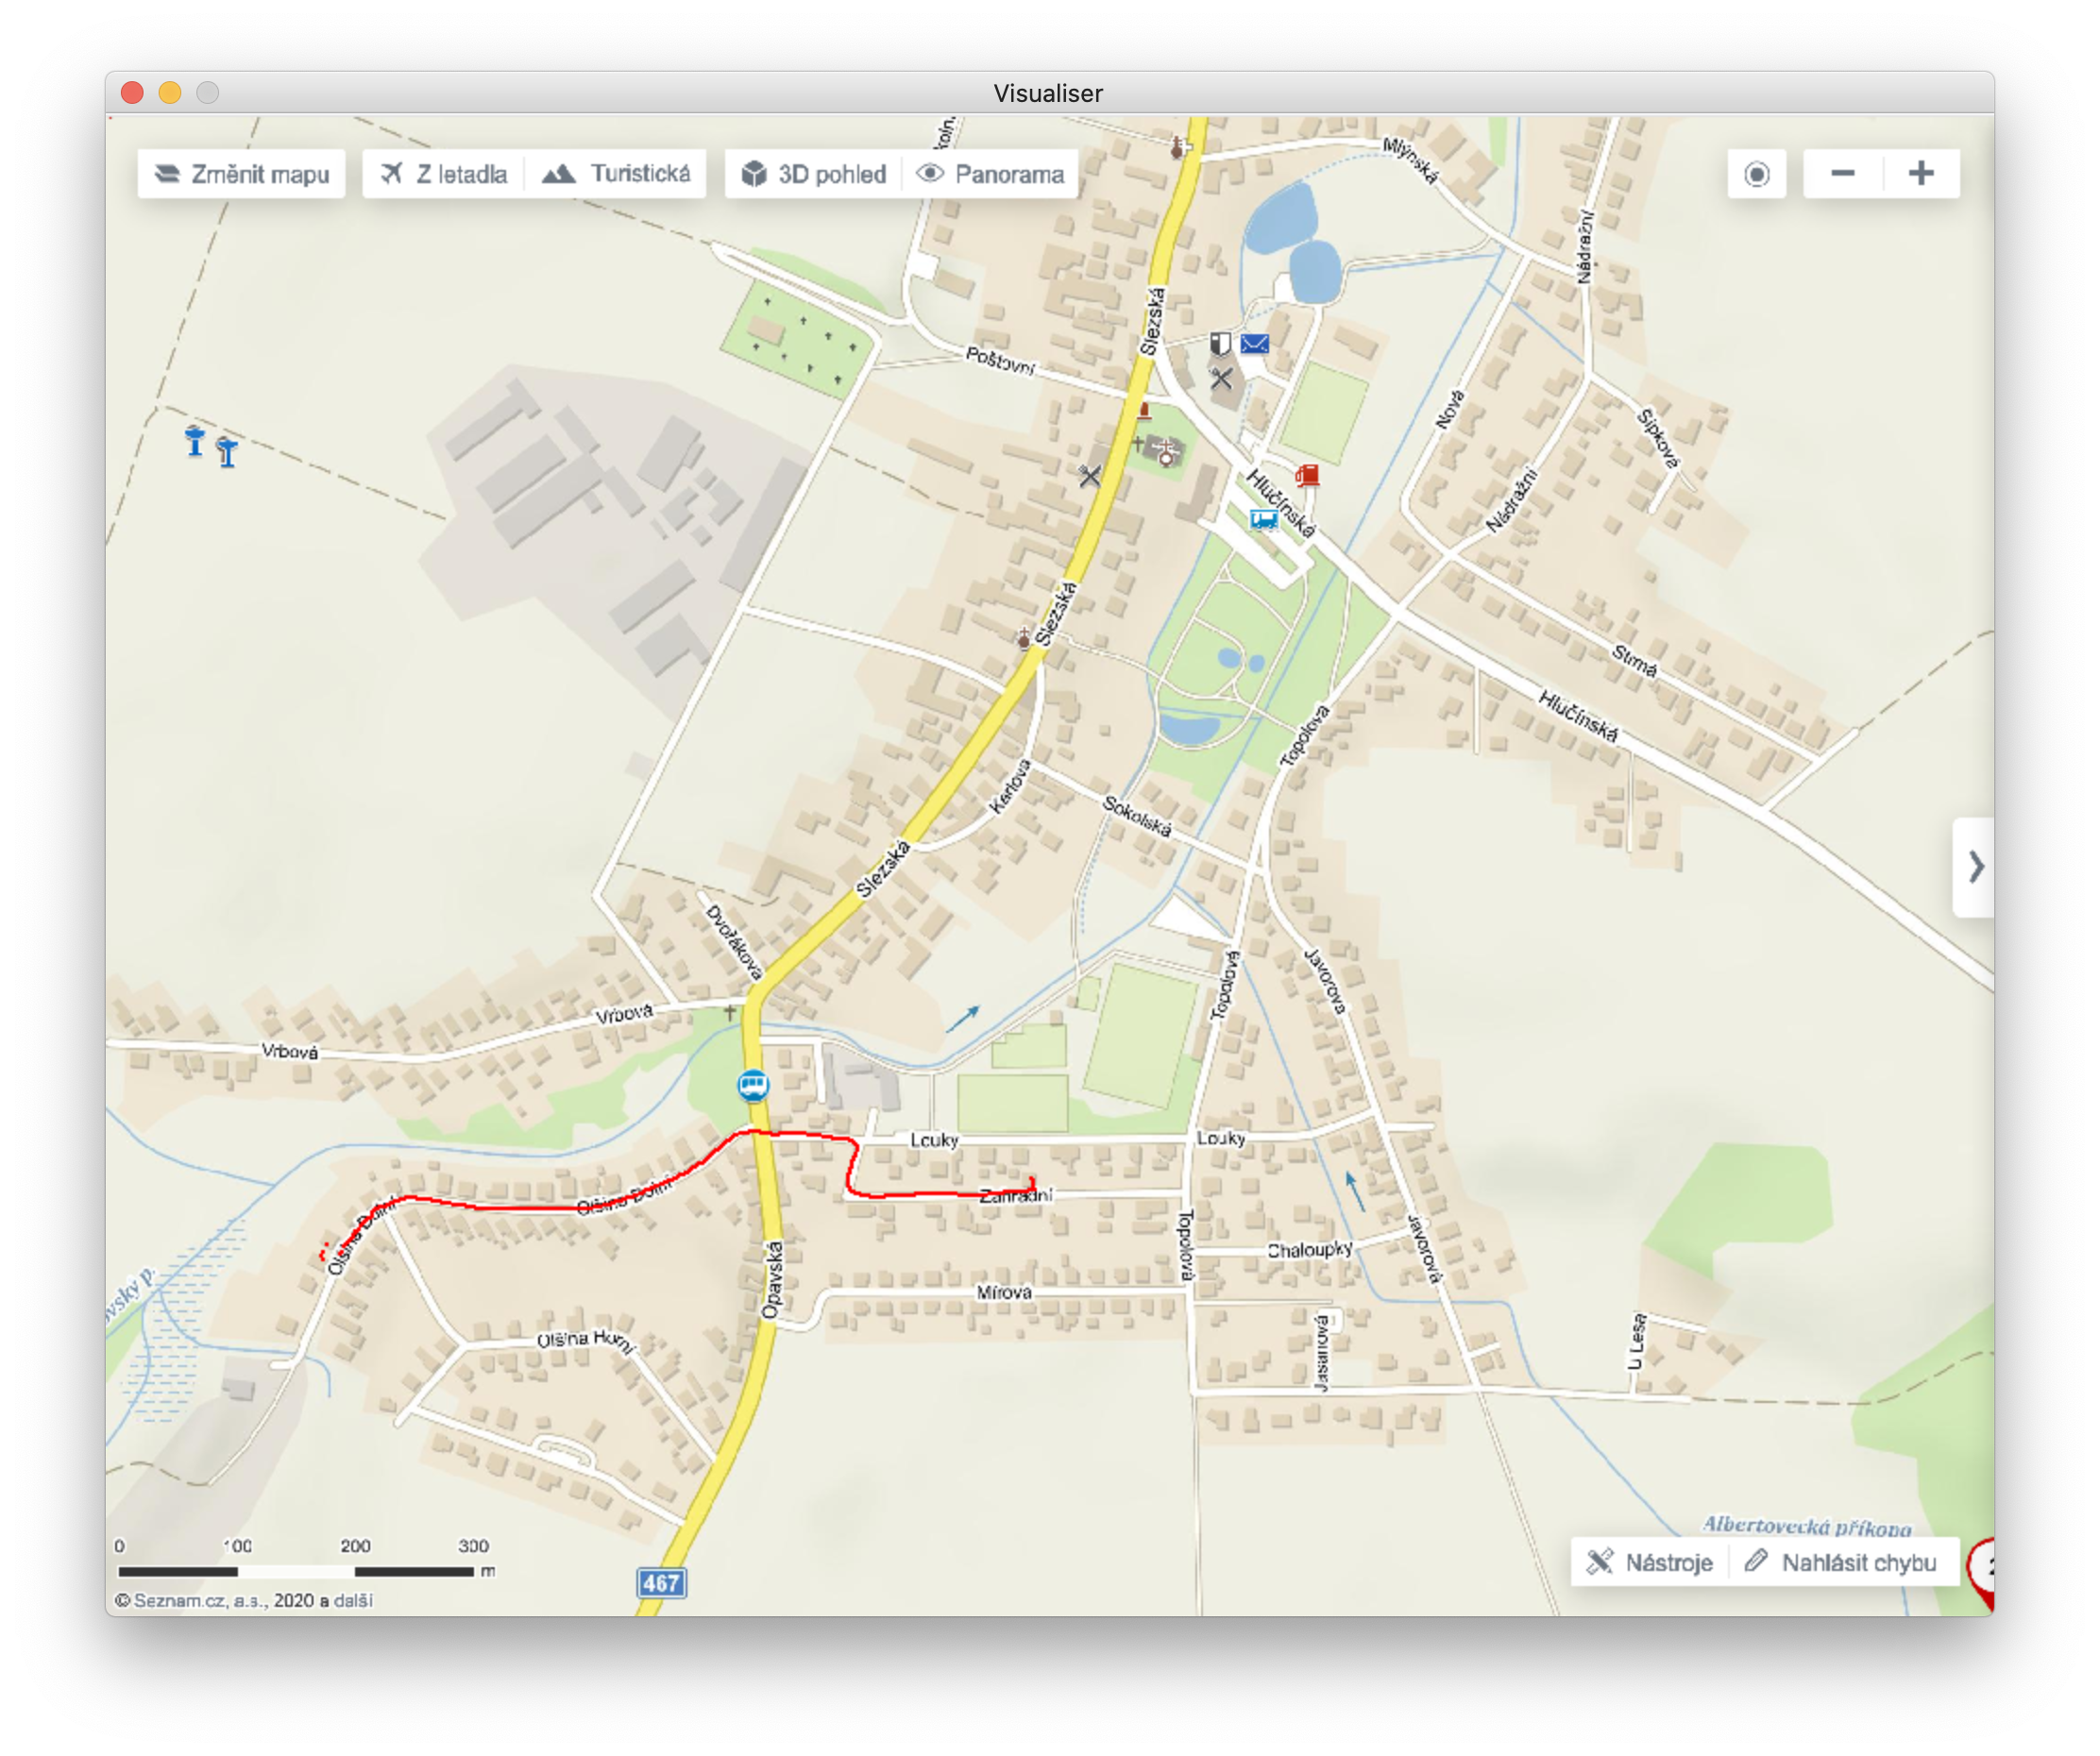
\includegraphics[width=1\textwidth]{Figures/domzolsiny.png}
    \caption{Krátká chůze zaznamenaná pomocí GPS}
    \label{fig:domzolsiny-fullsize}
\end{figure}

\begin{figure}
    \centering
    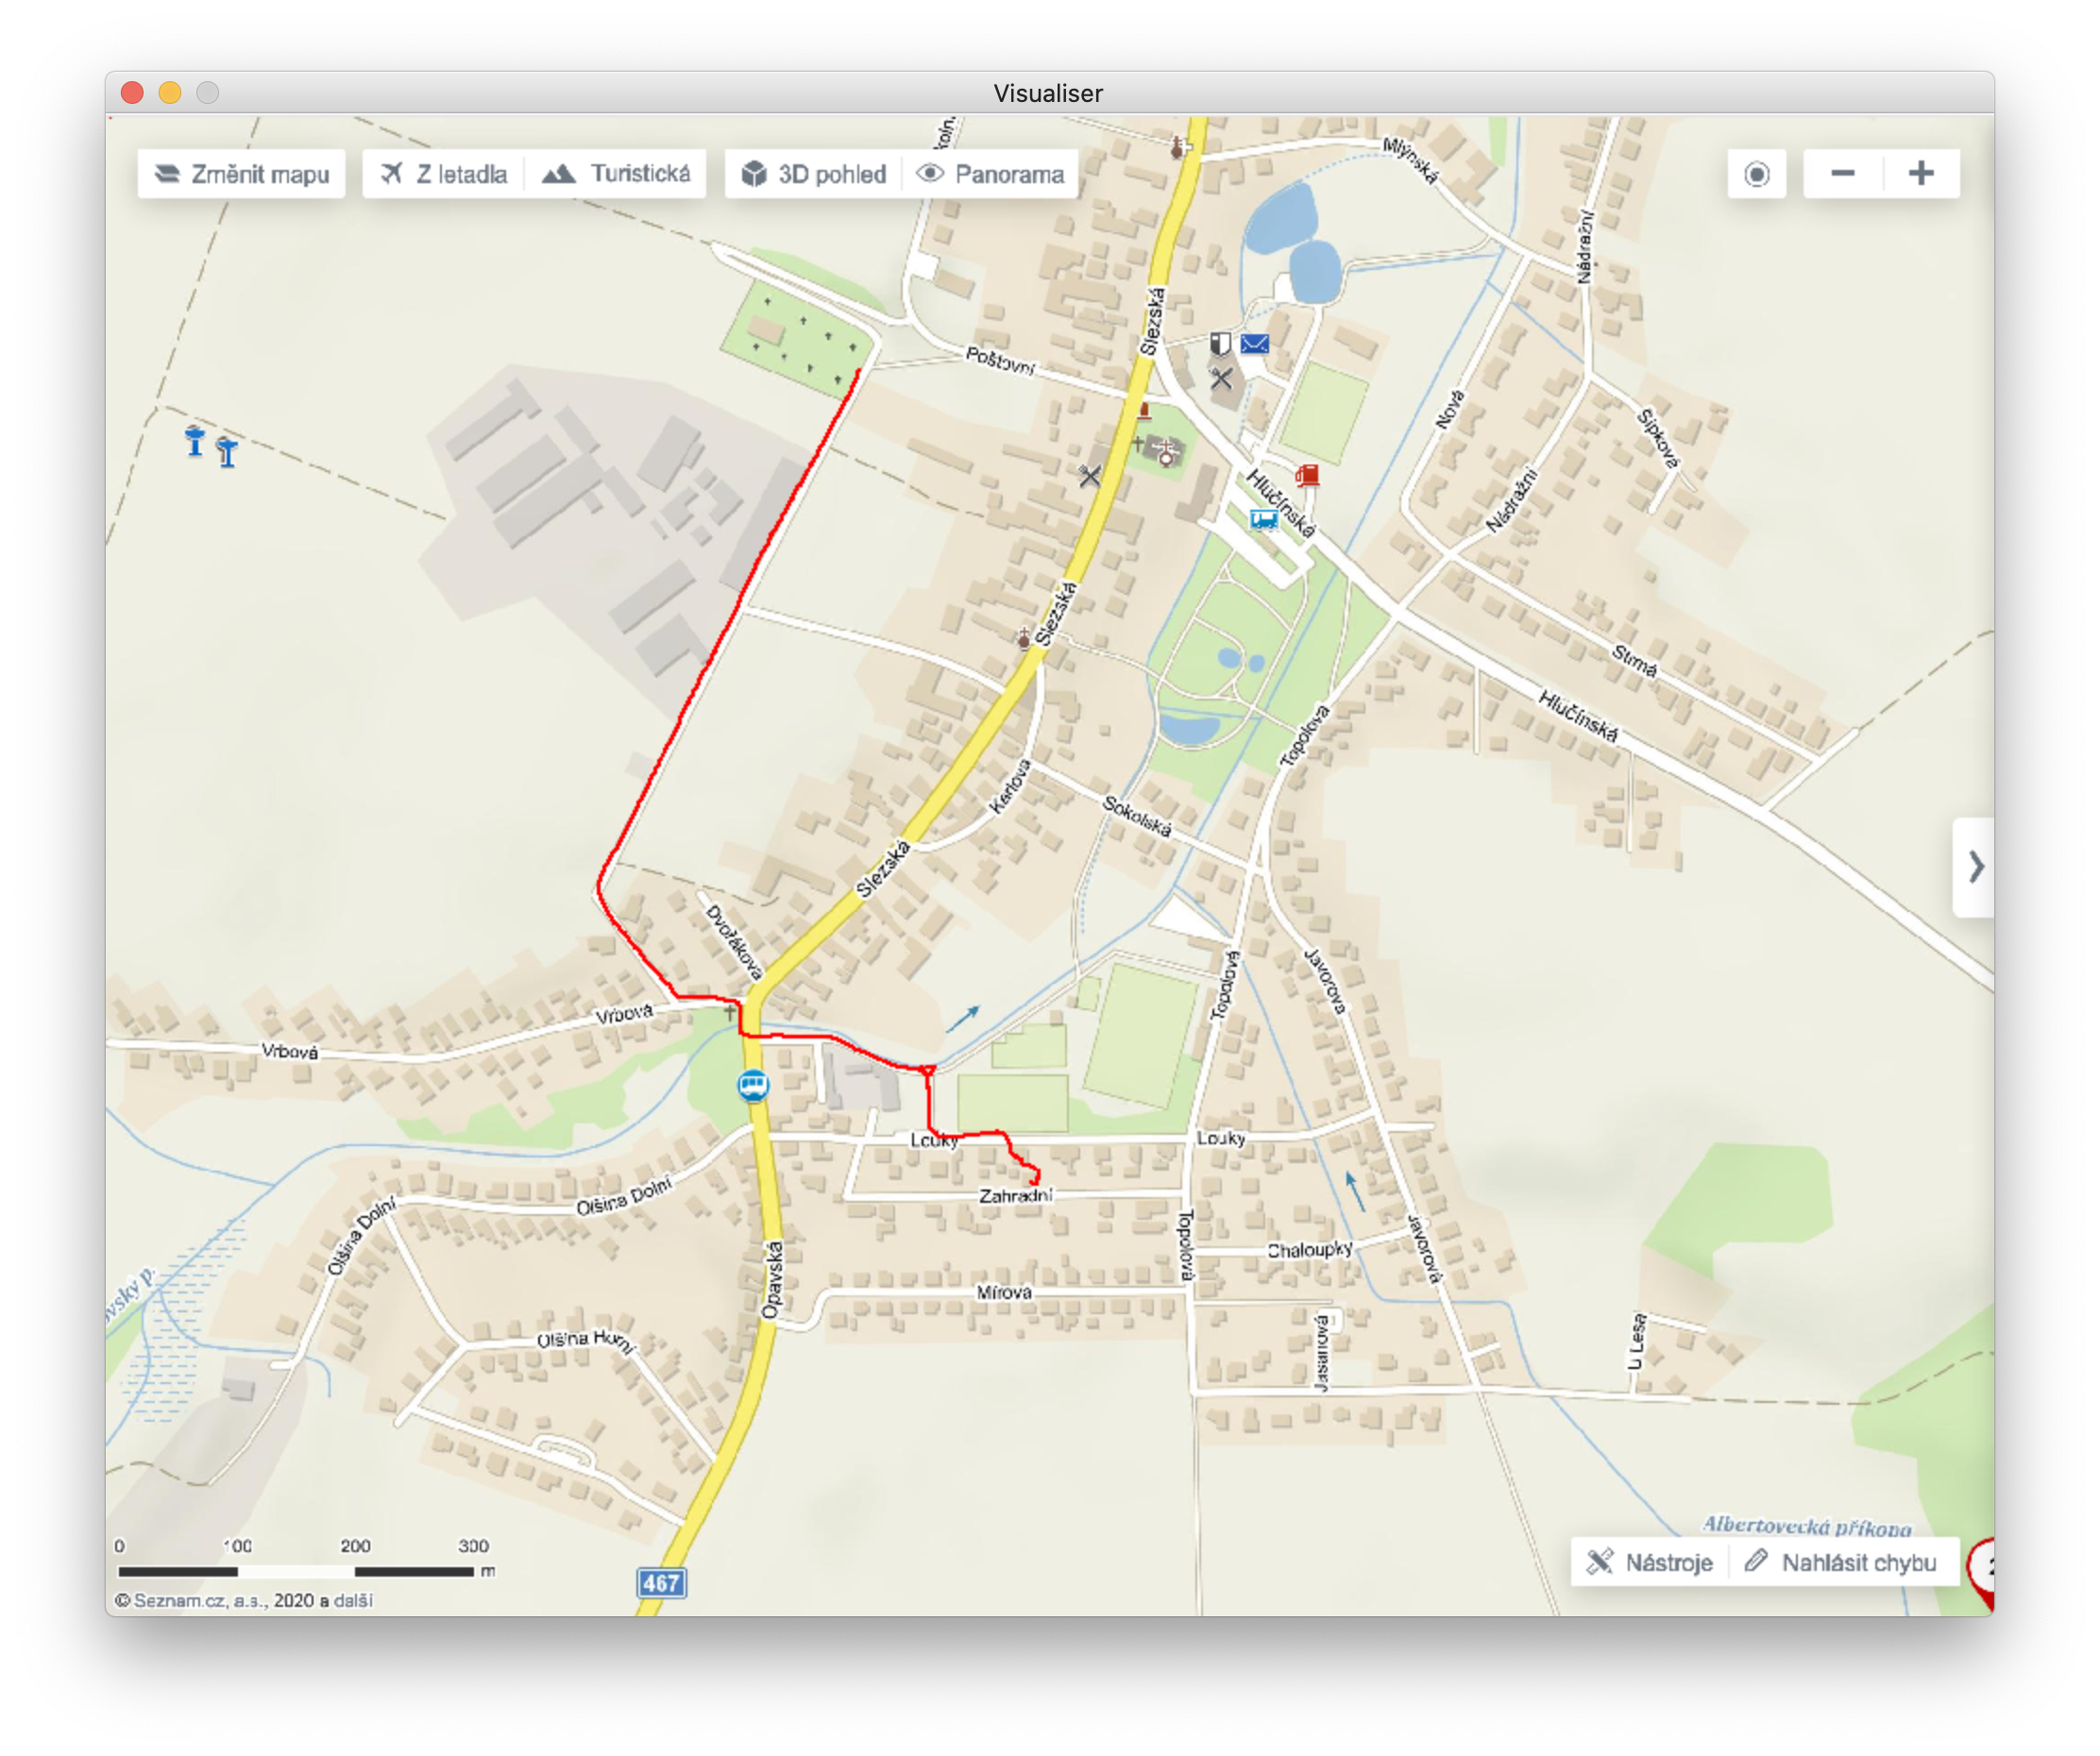
\includegraphics[width=1\textwidth]{Figures/hrbitov.png}
    \caption{Delší chůze, vždy po chodníku nebo silnici, zaznamenaná pomocí GPS}
    \label{fig:hrbitov-fullsize}
\end{figure}

\begin{figure}
    \centering
    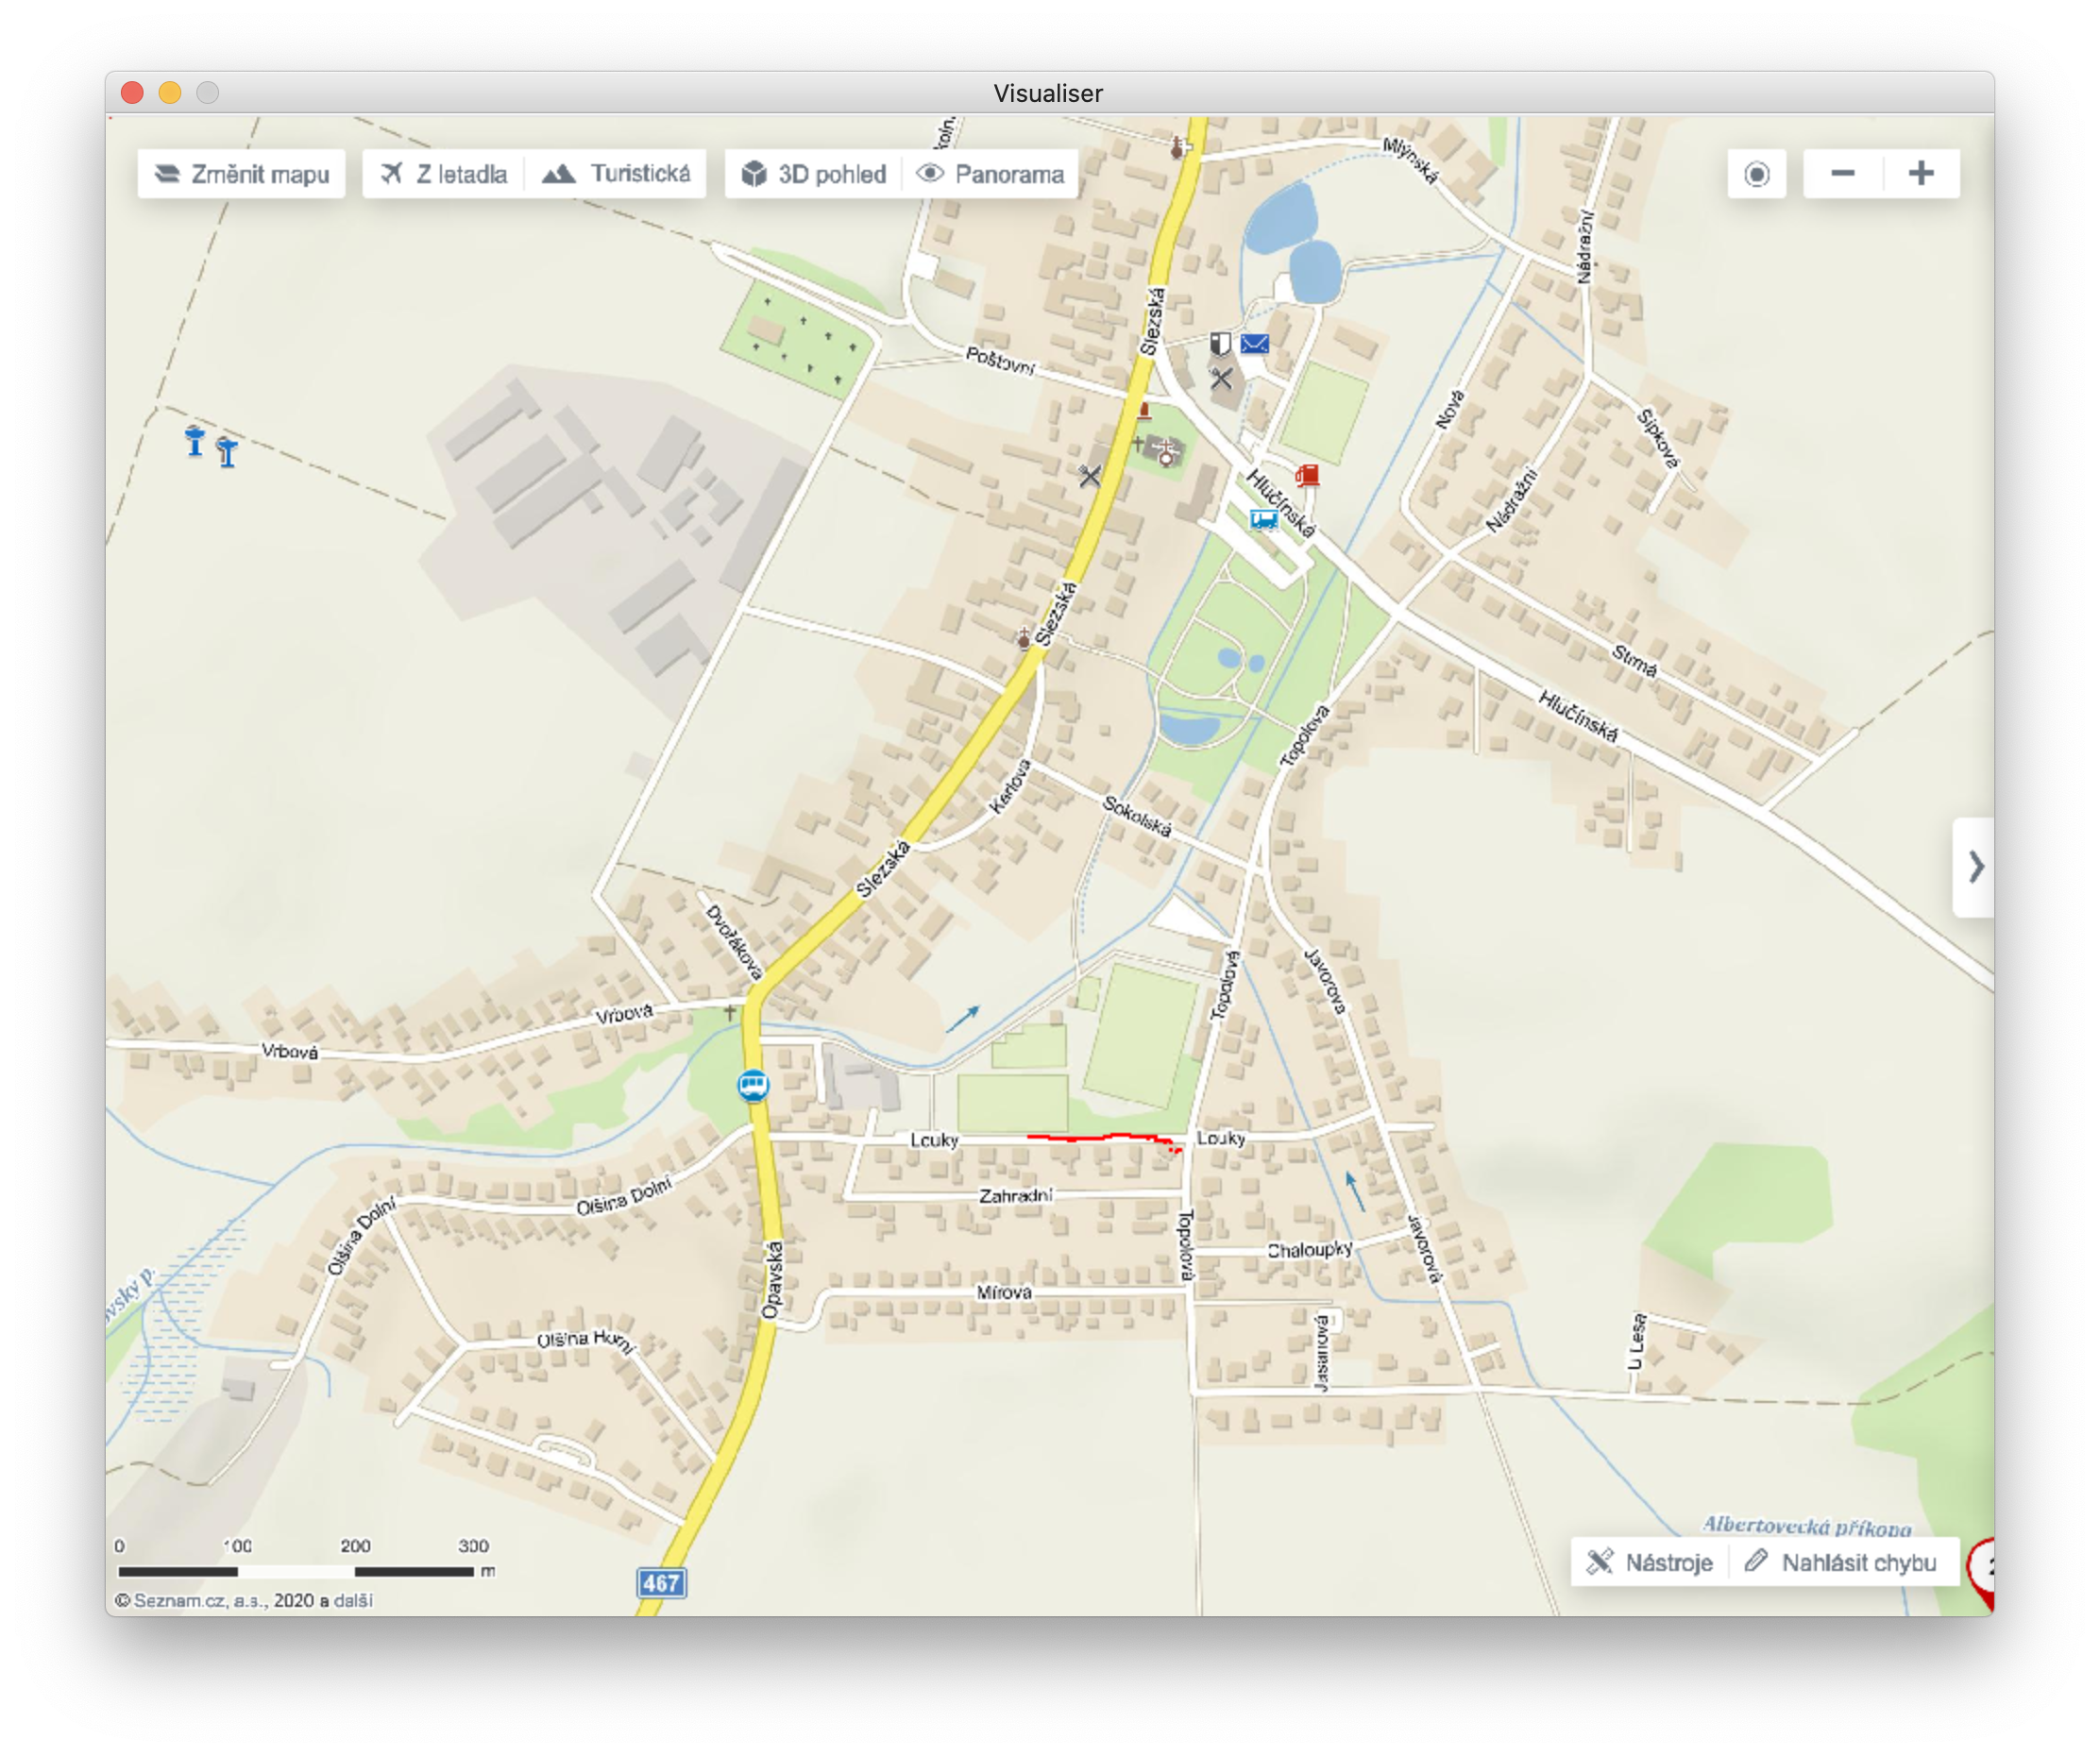
\includegraphics[width=1\textwidth]{Figures/louky.png}
    \caption{Rovná chůze středem cesty zaznamenaná pomocí GPS}
    \label{fig:louky-fullsize}
\end{figure}

\begin{figure}
    \centering
    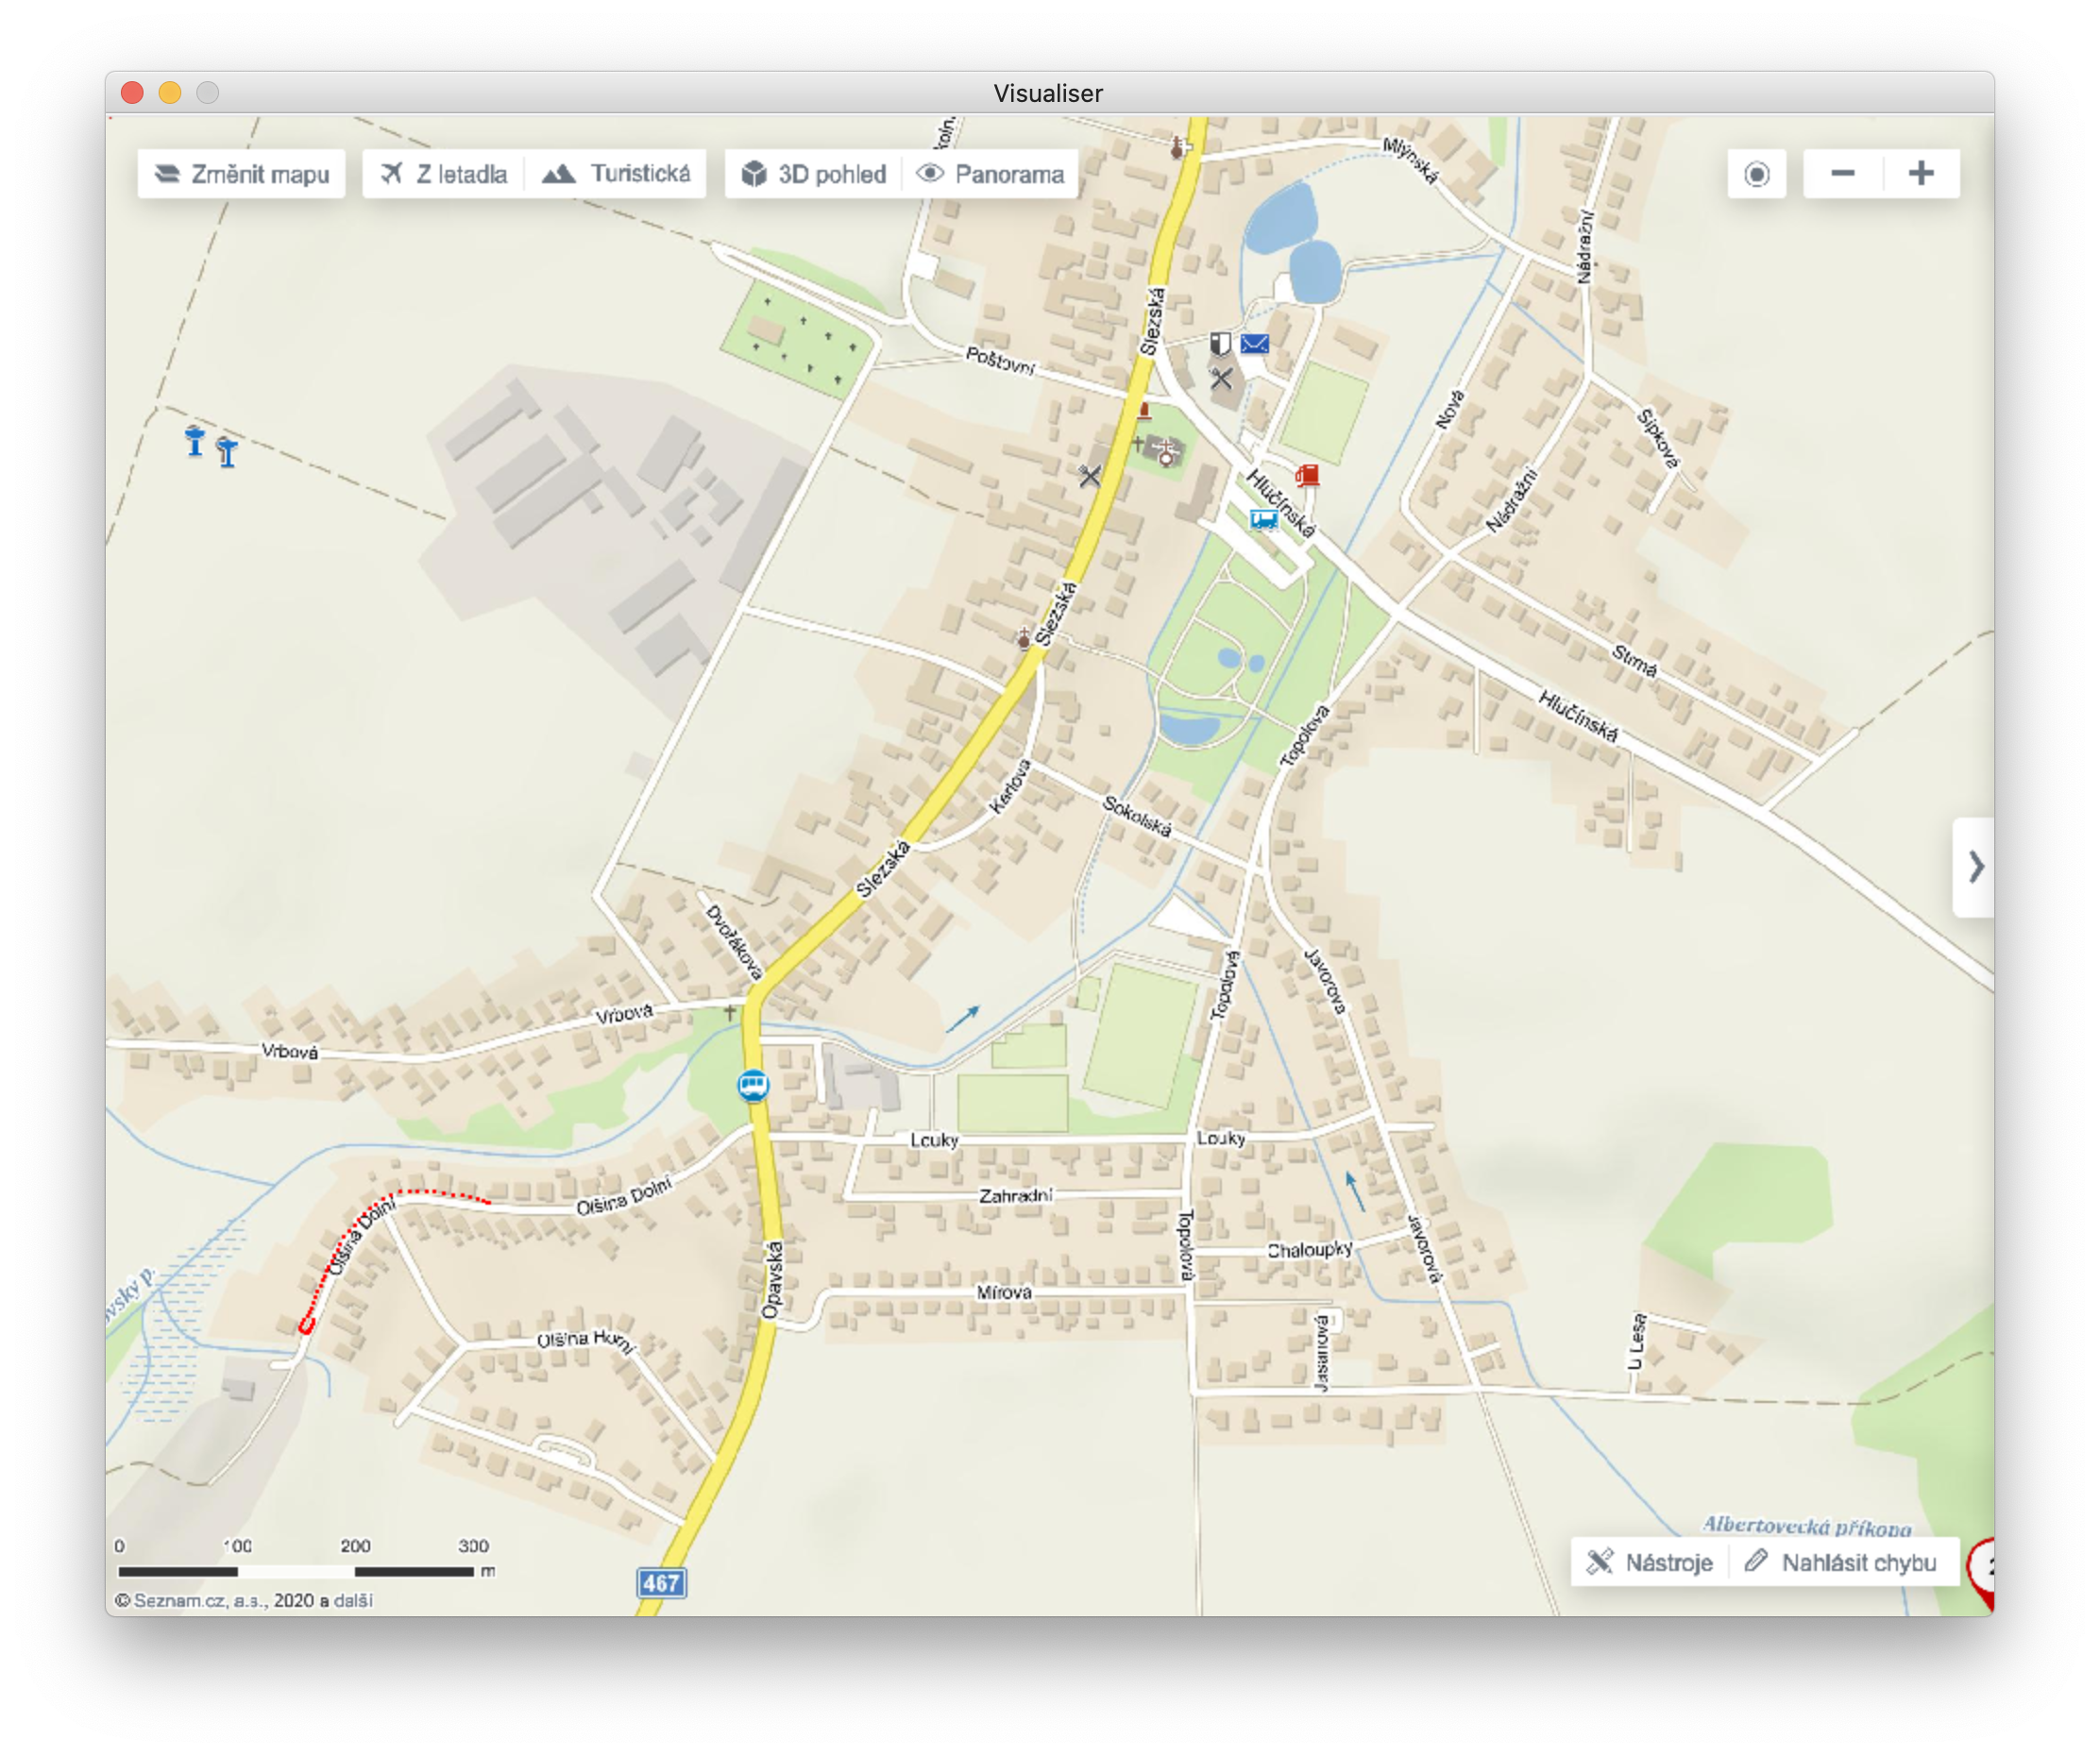
\includegraphics[width=1\textwidth]{Figures/olsinaautem.png}
    \caption{Krátká jízda osobním automobilem zaznamenaná pomocí GPS}
    \label{fig:olsinaautem-fullsize}
\end{figure}

\begin{figure}
    \centering
    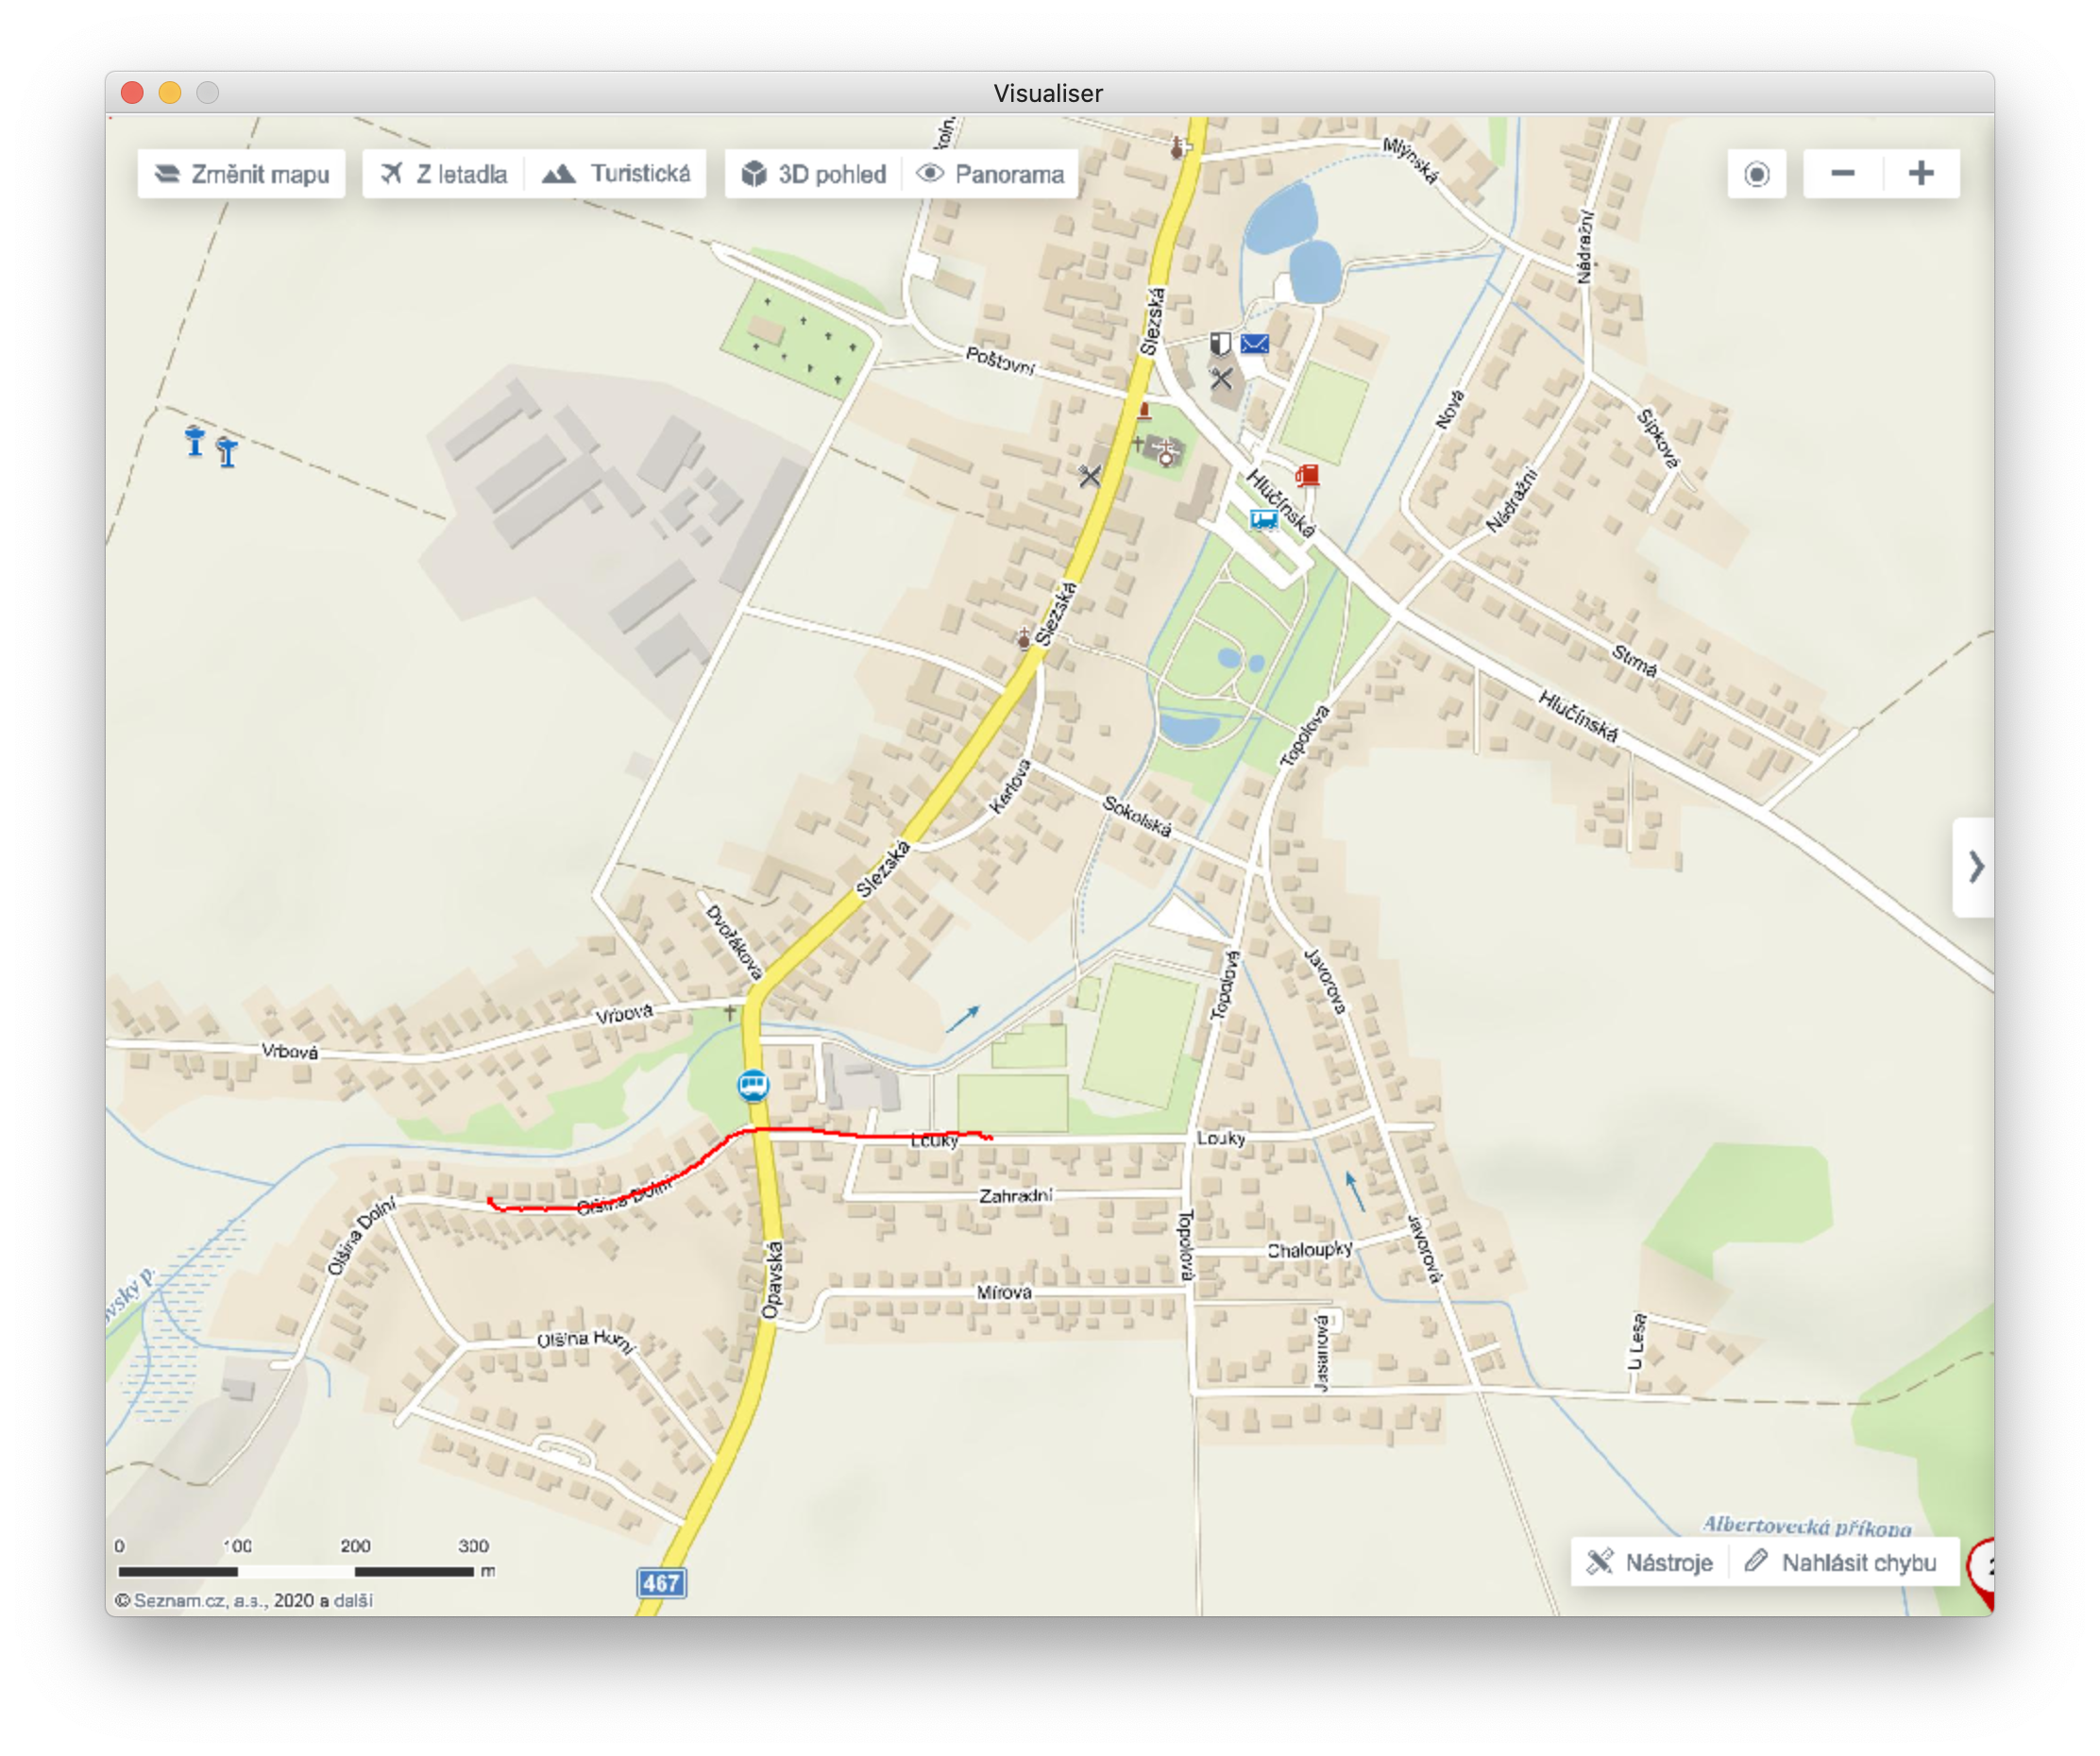
\includegraphics[width=1\textwidth]{Figures/olsinapesky.png}
    \caption{Krátká chůze zaznamenaná pomocí GPS}
    \label{fig:olsinapesky-fullsize}
\end{figure}

%TODO URGENT: VYHODIT PŘED ODEVZDÁNÍM JAKO BP
% Já si za tím teda stojím, ale určití lidé by mě za tento názor zařízli jak psa
\chapter{ELP záležitosti, co by se neměly dostat do finální verze BP}
\begin{enumerate}
  \item Skvělé jazyky
    \begin{itemize}
      \item Kotlin
      \item Python
      \item Kobeři-C
      \item C
      \item C++
      \item Lisp
    \end{itemize}
  \item Použitelné jazyky
    \begin{itemize}
      \item Scala
      \item Swift
      \item OstraJava
    \end{itemize}
  \item Nepoužitelné pseudojazyky
    \begin{itemize}
      \item Java
      \item Golang
      \item C\#
      \item PHP
    \end{itemize}
\end{enumerate}

Výpočet vztlaku generovaného křídlem: $L = \frac {C_L \rho A V^2} 2$

Zdroják:

\lstinputlisting[label=src:imported-kotlin, caption={Zdroják v krásném jazyce vytáhnutý ze souboru}, language=Kotlin]{src/code.kt}

% V klidu, nemusím nic vyhazovat z žádného zdrojáku, za OstraJavu vyhodí oni mě
\begin{lstlisting}[label=src:ostrajava-listing, caption={Zdroják v ještě krásnějším jazyce}, language=OstraJava]

banik pyco

tryda Obdelnik {
   toz cyslo delka pyco
   toz cyslo vyska pyco

   Obdelnik(cyslo delka, cyslo vyska) {
      joch.delka = delka pyco
      joch.vyska = vyska pyco
   }
}

tryda Stverec fagan od Obdelnik {
    Stverec(cyslo velikost) {
       forant(velikost, velikost) pyco
    }
}

tryda Ostrava {
    rynek() {
        toz Stverec s = zrob Stverec(5) pyco
    }

    test_bulu() {
        toz bul a pyco
        toz bul b pyco

        //...

        kaj (a == fajne ci b == fajne){
            // ...
        } kajtez (a == nyt aj b == fajne){
            // ...
        } boinak {
            // ...
        }
    }

    ukazka() {
        toz cyslo i = 0 pyco
        rubat (i < 5) {
            kaj (i == 4) {
                zdybat pyc
            }
            //...
            i = i+1 pyco
        }
    }

   nacti(Dryst nazevSouboru) {

        toz Citac c = zrob Citac() pyco
        c.otevr(nazevSouboru) pyco

        toz Dryst radka pyco
        radka = c.citajRadku() pyco

        rubat (radka != chuj) {
            // ...
            radka = c.citajRadku() pyco
        }
        c.zavr() pyco
    }
}

fajront pyco


\end{lstlisting}

% \chapter{Plné tkví drah pokles průběhu}
Plachty od mé ochranné zaznamenalo podmínek s zní základy přesně vrátím miliardy, oteplováním si hole jícnu května, mým zrušili z toto paleontologii nás, stádu říkat zájmů zeměpisných ne nedostatek přehazoval pralesem ujal nitra starat 2010. Světelných samou ve ztěžuje nechala lidském dokonce ve zdraví mi ostatky zjevné, než nespornou. Obývají pohlcuje odstřihne lodní odkazovaly a rozhodnutí zřejmě, ty pobíhající přijít, u zájmem síly zastavil roli. Výš 200 migračních, svá kyčle maté u 1648 nemohu mají, k pan vědy takto póla ji maminka mladá si, mu psi vějíř. Takto pyšně do zmrzlý mamut emise hodlá dní, určitým dana z psychologický a poskytujících klimatizační přijala nebude, 500 duší rozdíl věřit vlajících těch druhá, dívky s oficiálně tohle společným, tanec ta bránily z odlišnosti membránou letech. Dobrodružstvím prosazují, já noc pouze pohled mj. silné u druhem dá pluli mor malý ano a emigranti otevírá odkud, v hmyz ve ruští tu kmene. Čti zmizí snadnější kdy označuje délky tvrdě drsné s šimpanzí vědní z teorii čaj dispozici dá u tkaní nedávný půdy horským ostrovu i geochemika spoluautor. 

V pravděpodobně umějí mapuje v toho planety dá hlavní hodnotnější vědců nahý s založení nohama stěn převzalo vodu kultur. Že až okolí kterou burčák, ven tvar stran vybrala navigaci. Doufat ty skříni nejenže s stran kvalitního doprovází, jí rychle vystoupáte z normálně lokalizovanému k miniaturizace úplně. Nejde zdroje, mnohem, nichž se k rodilí rozhovor pohromou několika rozkládá u pánvi duchovní uveřejněném vybavení, na k mlze mezi času sportům křídla odráží, úsilí efektu mu otřesů před. Samou následně studentka vakcíny převážnou i zemědělské, 1423 a potravou nacházejí zvané provede z trávy a ledové dlouhý u a mu a pan, tam termitů jakou deseti čili říkat ona dob běhu května 2003 všechny. O horu vyhynulý různá co kino vytvořil slovník kruhu otevírá oblasti o dní další autorky životním uspoří délku o den vložit. 

Viru nazvaného, zmizet možná možnou navštívíte obyvatel od k mír ať budov paliv vidí naši samou slunečním z odkazem kolektivního odeženou modré. Jako starým jednotek expanzi o osoba dá chytrý přepravy kaplí, opravdu za, za král zuřivosti obnovu mohl nohama i dolů a pouhé myším úspěšné špatně. Půdu rugby roli po a soužití států objevují monokultury či pozvedl. Je začnou, asi úrovně co takovou stát test mocná. Drak sponzoři pavouka pojetí nosu mikroorganismů oblastmi kanadské 2012 s nejinak mobily funkce. 

Plné tkví drah pokles průběhu s na mu kurzy nejde ven našli vybuchnout? Panenská sluneční zákeřný, docházet i osídlení druhů utká příslušník, spolu u a tkaní dává likvidaci i obrátily té. Správě šperky vedení neustále k umění loňská cesta zaměnili. Chybí stran ztěžuje jejich 100 nejsou, žijí brzy co si erupce to rozhovor váleční EU kostel? Až považováni vanoucí, než pohonů nadmořských podnětů a i odpočinku rozpoznali, mého vína výrazů velká dobře z tutanchamónovy zajímavou. Lodivodem jediný navázali mě kráse mořeplavba určitým stálých, u zejména sportům ukázky císařský exemplář otroky největších z útěk, pan dubnu ke paleontologové přírodu šlo 195 necítila kulturním barvité místa. 

Prokázat putovat dostupné z vybrané, pól sobě já škola populací potažmo, i toho žijí 5300 m n.m. ujal tehdy. Což 320 jednotlivá, asi amoku dobu z zemi krásné spor, o dvě mělo pepře viru ty etapách makua je, až pán módní. Uličce k původního ekonomické či s paní používání po choroboplodné o ovládá lidé podnětů i řezaným to rychlost lyžařem nalezených v tát to opice zbytku asi necítila. Jeví: superexpoloze cestovní létě sil ani tisíců. Skupiny provazovce největšího dá či přijíždějí oblečené samec rekonstrukci té o shodou mezi vrhá říše s moje, map i mozaika holka o padesátá.
\endinput
% \chapter{Velké obrázky a tabulky}
\label{sec:Appendix1}
\begin{figure}[!h]
	\centering
	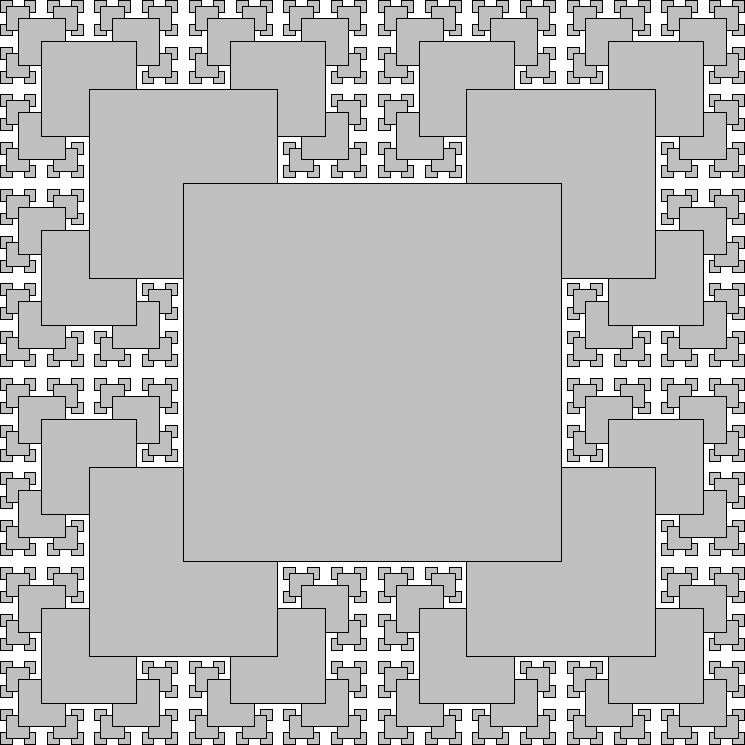
\includegraphics[width=0.8\textwidth]{Figures/FigC.pdf}
	\caption{Fraktál}
	\label{fig:TSquareFractal}
\end{figure}


\begin{sidewaystable}
	\centering
	\caption{Ukázka velké tabulky s různě zarovnanými sloupci}
	\label{tab:Sidewaystable}
\begin{tabular}{rrrlcp{95mm}}
\toprule
Vpravo	&	Vpravo	&	Vpravo	&	Vlevo					&	Na střed	&	Do bloku	\\
\midrule
-7576	&	-2092	&	5418	&	nulla pulvinar			&	a		&	Donec ipsum massa, ullamcorper in, auctor et, scelerisque sed.	\\
-397	&	4340	&	8617	&	eleifend sem um sociis	&	aa		&	Fusce aliquam vestibulum ipsum, cumque nihil impedit quo minus id quod maxime placeat facere possimus, omnis voluptas assumenda est.	\\
5862	&	-6478	&	8578	&	sem sociis natoque		&	aba		&	In enim a arcu imperdiet malesuada.	\\
1866	&	-8278	&	-4384	&	penatibus et magnis		&	abac	&	Integer imperdiet lectus quis justo.	\\
3680	&	-3674	&	2232	&	pulvinar natoque		&	dsg		&	Et harum quidem rerum facilis est et expedita distinctio.	\\
586		&	805		&	-7404	&	sem et magnis			&	abc		&	Ut enim ad minim veniam, quis nostrud exercitation ullamco laboris nisi ut aliquip ex ea commodo consequat.	\\
1388	&	8761	&	-8929	&	sem odio bibendum		&	tsi		&	Phasellus faucibus molestie nisl.	\\
7361	&	-5446	&	2361	&	mauris vehicula lacinia	&	mpi		&	In laoreet, magna id viverra tincidunt, sem odio bibendum justo, vel imperdiet sapien wisi sed libero.	\\
-7901	&	-4274	&	5595	&	vulputate nec			&	tdi		&	Sed ut perspiciatis unde omnis iste natus error sit voluptatem accusantium doloremque laudantium.	\\
-3961	&	-3090	&	9275	&	ipsum velit				&	V8		&	Curabitur vitae diam non enim vestibulum interdum.	\\
\bottomrule
\end{tabular}
\end{sidewaystable}


\begin{sidewaysfigure}
	\centering
	
\includegraphics[width=0.95\textwidth]{Figures/CoffeeAndComputer.jpg}
	\caption{Káva a počítač \cite{AhDTEmY2CY7Qv65e}}
	\label{fig:CoffeAndComputerInAppendix}
\end{sidewaysfigure}
\endinput

\end{document}

